\documentclass[a4paper,12pt]{report}
%\documentclass[aps,twocolumn,secnumarabic,balancelastpage,amsmath,amssymb,nofootinbib,floatfix]{revtex4-1}
\usepackage[utf8]{inputenc}
\usepackage[a4paper, total={6in, 8in}]{geometry}
\usepackage{graphicx}
\usepackage{mathrsfs}
\usepackage{amsmath}
\usepackage{amsfonts}
\usepackage{sidecap}
\usepackage{setspace}
\usepackage{fancyvrb}

\renewcommand{\thesection}{\arabic{section}}

\begin{document}

\title{Numerically Modeling Gravitationally Bound Systems}
\author{Noah Green \\ Michigan State University}
%\affiliation{Michigan State University}
\date{April 1, 2016}
\maketitle
\begin{abstract}
The RK4 and Verlet algorithms for calculating the solutions to ordinary differential equations are used here to calculate the orbits of various gravitationally bound systems resembling the solar system. It was found that the RK4 algorithm is more accurate, but the Verlet algorithm is easier to implement. Additionally, systems that have many bodies that move on different timescales become difficult to model, requiring many more time steps to accurately model objects moving on a short timescale (e.g. Mercury) than is necessary to accurately model objects moving on a long timescale (e.g. Pluto). This was remedied in a model solar system by treating the inner and outer solar systems separately, and ignoring the negligible effect of the gravitational force due to the first four planets on the outer four planets and Pluto.
\end{abstract}

\doublespacing
\section{Introduction}\label{sec:intro}
Modeling the gravitational force has many applications, from space travel to astronomy. I will discuss how to use the Runge-Kutta and Verlet algorithms to numerically calculate the motion of model solar systems due to classical gravitational interactions. In section \ref{sec:diffeq}, I cover the equations used to model gravitational interactions. In section \ref{sec:alg}, I discuss how these equations can be solved numerically. In section \ref{sec:ss}, I show these algorithms applied in different situations. Finally, in section \ref{sec:conclude}, I summarize the conclusions of this study.

\section{Differential Equations}\label{sec:diffeq}
The force due to gravity between two objects can be calculated using Newton's law of gravitation:
\begin{equation}\label{eq:gravitation}
 F_G = \frac{GMm}{r^2}
\end{equation}
where $G$ is the universal gravitational constant, $M$ and $m$ are the masses of the two object, and $r$ is the distance between them. Newton's second law, $F = ma$ gives us that 
\begin{equation}\label{eq:nsl}
 \frac{d^2x}{dt^2} = \frac{F_{G,m,x}}{m}
\end{equation}
with similar equations for $y$ and $z$. In order to use the algorithms, these equations must be rewritten as a set of coupled first order ordinary differential equations


\section{Algorithms}\label{sec:alg}

\subsection{RK4}

\singlespacing
\begin{Verbatim}[fontsize=\small]
   for( int i = 1; i <= _Ntime; i++ ){
    vector< vector< double > > k1, k2, k3; 
    for( unsigned int iPlanet = 0; iPlanet < GetN(); iPlanet++ ){
    
    ... Calculate k1, k2, k3, k4...
    
    	_vPlanets.at(iPlanet).SetX(_vPlanets.at(iPlanet).X(i-1)
				   +(k1.at(iPlanet).at(0)
				   +2.*k2.at(iPlanet).at(0)
				   +2.*k3.at(iPlanet).at(0)
				     +k4i.at(0))/6.,i);
	_vPlanets.at(iPlanet).SetY(_vPlanets.at(iPlanet).Y(i-1)
				   +(k1.at(iPlanet).at(1)
				   +2.*k2.at(iPlanet).at(1)
				   +2.*k3.at(iPlanet).at(1)
				     +k4i.at(1))/6.,i);
	_vPlanets.at(iPlanet).SetZ(_vPlanets.at(iPlanet).Z(i-1)
				   +(k1.at(iPlanet).at(2)
				   +2.*k2.at(iPlanet).at(2)
				   +2.*k3.at(iPlanet).at(2)
				     +k4i.at(2))/6.,i);
	_vPlanets.at(iPlanet).SetVx(_vPlanets.at(iPlanet).Vx(i-1)
				    +(k1.at(iPlanet).at(3)
				    +2.*k2.at(iPlanet).at(3)
				    +2.*k3.at(iPlanet).at(3)
				      +k4i.at(3))/6.,i);
	_vPlanets.at(iPlanet).SetVy(_vPlanets.at(iPlanet).Vy(i-1)
				    +(k1.at(iPlanet).at(4)
				    +2.*k2.at(iPlanet).at(4)
				    +2.*k3.at(iPlanet).at(4)
				      +k4i.at(4))/6.,i);
	_vPlanets.at(iPlanet).SetVz(_vPlanets.at(iPlanet).Vz(i-1)
				    +(k1.at(iPlanet).at(5)
				    +2.*k2.at(iPlanet).at(5)
				    +2.*k3.at(iPlanet).at(5)
				      +k4i.at(5))/6.,i);
      }
    }
  }
\end{Verbatim}
\doublespacing


\subsection{Verlet}

\begin{Verbatim}[fontsize=\small]
void SolarSystem::Verlet(){
  _solved = true;
  // make force variables in this scope so they persist through loops
  vector<double> Fx,Fy,Fz;
  vector<double> fx,fy,fz;
  double f_x,f_y,f_z;
  for( unsigned int fi = 0; fi < GetN(); fi++ ){
    TotalForce(fi,0,f_x,f_y,f_z);
    Fx.push_back(f_x);
    Fy.push_back(f_y);
    Fz.push_back(f_z);
    fx.push_back(f_x);
    fy.push_back(f_y);
    fz.push_back(f_z);
  }

  for( int i = 1; i <= _Ntime; i++){
    for( unsigned int iPlanet = 0; iPlanet < GetN(); iPlanet++ ){
      if(_vPlanets.at(iPlanet).Fixed()){
	_vPlanets.at(iPlanet).AddCoordinates(i*_step,
					     _vPlanets.at(iPlanet).X(i-1),
					     _vPlanets.at(iPlanet).Y(i-1),
					     _vPlanets.at(iPlanet).Z(i-1),
					     _vPlanets.at(iPlanet).Vx(i-1),
					     _vPlanets.at(iPlanet).Vy(i-1),
					     _vPlanets.at(iPlanet).Vz(i-1));  
      }
      else{
	// advance spatial coordinates by one time step
	// set velocity to zero for now
	fx.at(iPlanet) = Fx.at(iPlanet);
	fy.at(iPlanet) = Fy.at(iPlanet);
	fz.at(iPlanet) = Fz.at(iPlanet);
	_vPlanets.at(iPlanet).AddCoordinates(i*_step,
					     _vPlanets.at(iPlanet).X(i-1)+ 
					     _step*_vPlanets.at(iPlanet).Vx(i-1)+
					     _step*_step*fx.at(iPlanet)/(2.*_vPlanets.at(iPlanet).M()),
					     _vPlanets.at(iPlanet).Y(i-1)+
					     _step*_vPlanets.at(iPlanet).Vy(i-1)+
					     _step*_step*fy.at(iPlanet)/(2.*_vPlanets.at(iPlanet).M()),
					     _vPlanets.at(iPlanet).Z(i-1)+
					     _step*_vPlanets.at(iPlanet).Vz(i-1)+
					     _step*_step*fz.at(iPlanet)/(2.*_vPlanets.at(iPlanet).M()),
					     0.,0.,0.);
      }
    }
    for( unsigned int iPlanet = 0; iPlanet < GetN(); iPlanet++){
      if( !_vPlanets.at(iPlanet).Fixed() ){
	// calculate force using new position coordinates
	TotalForce(iPlanet,i,Fx.at(iPlanet),Fy.at(iPlanet),Fz.at(iPlanet));
	// advance velocity coordinates by one step
	_vPlanets.at(iPlanet).SetVx(_vPlanets.at(iPlanet).Vx(i-1)+
				    _step*(fx.at(iPlanet)+Fx.at(iPlanet))/(2.*_vPlanets.at(iPlanet).M()),i);
	_vPlanets.at(iPlanet).SetVy(_vPlanets.at(iPlanet).Vy(i-1)+
				    _step*(fy.at(iPlanet)+Fy.at(iPlanet))/(2.*_vPlanets.at(iPlanet).M()),i);
	_vPlanets.at(iPlanet).SetVz(_vPlanets.at(iPlanet).Vz(i-1)+
				    _step*(fz.at(iPlanet)+Fz.at(iPlanet))/(2.*_vPlanets.at(iPlanet).M()),i);
	
      }
    }
  }
}
\end{Verbatim}

\section{The Solar System}\label{sec:ss}

\subsection{Earth-Sun only}

 \begin{SCfigure}
 \centering
   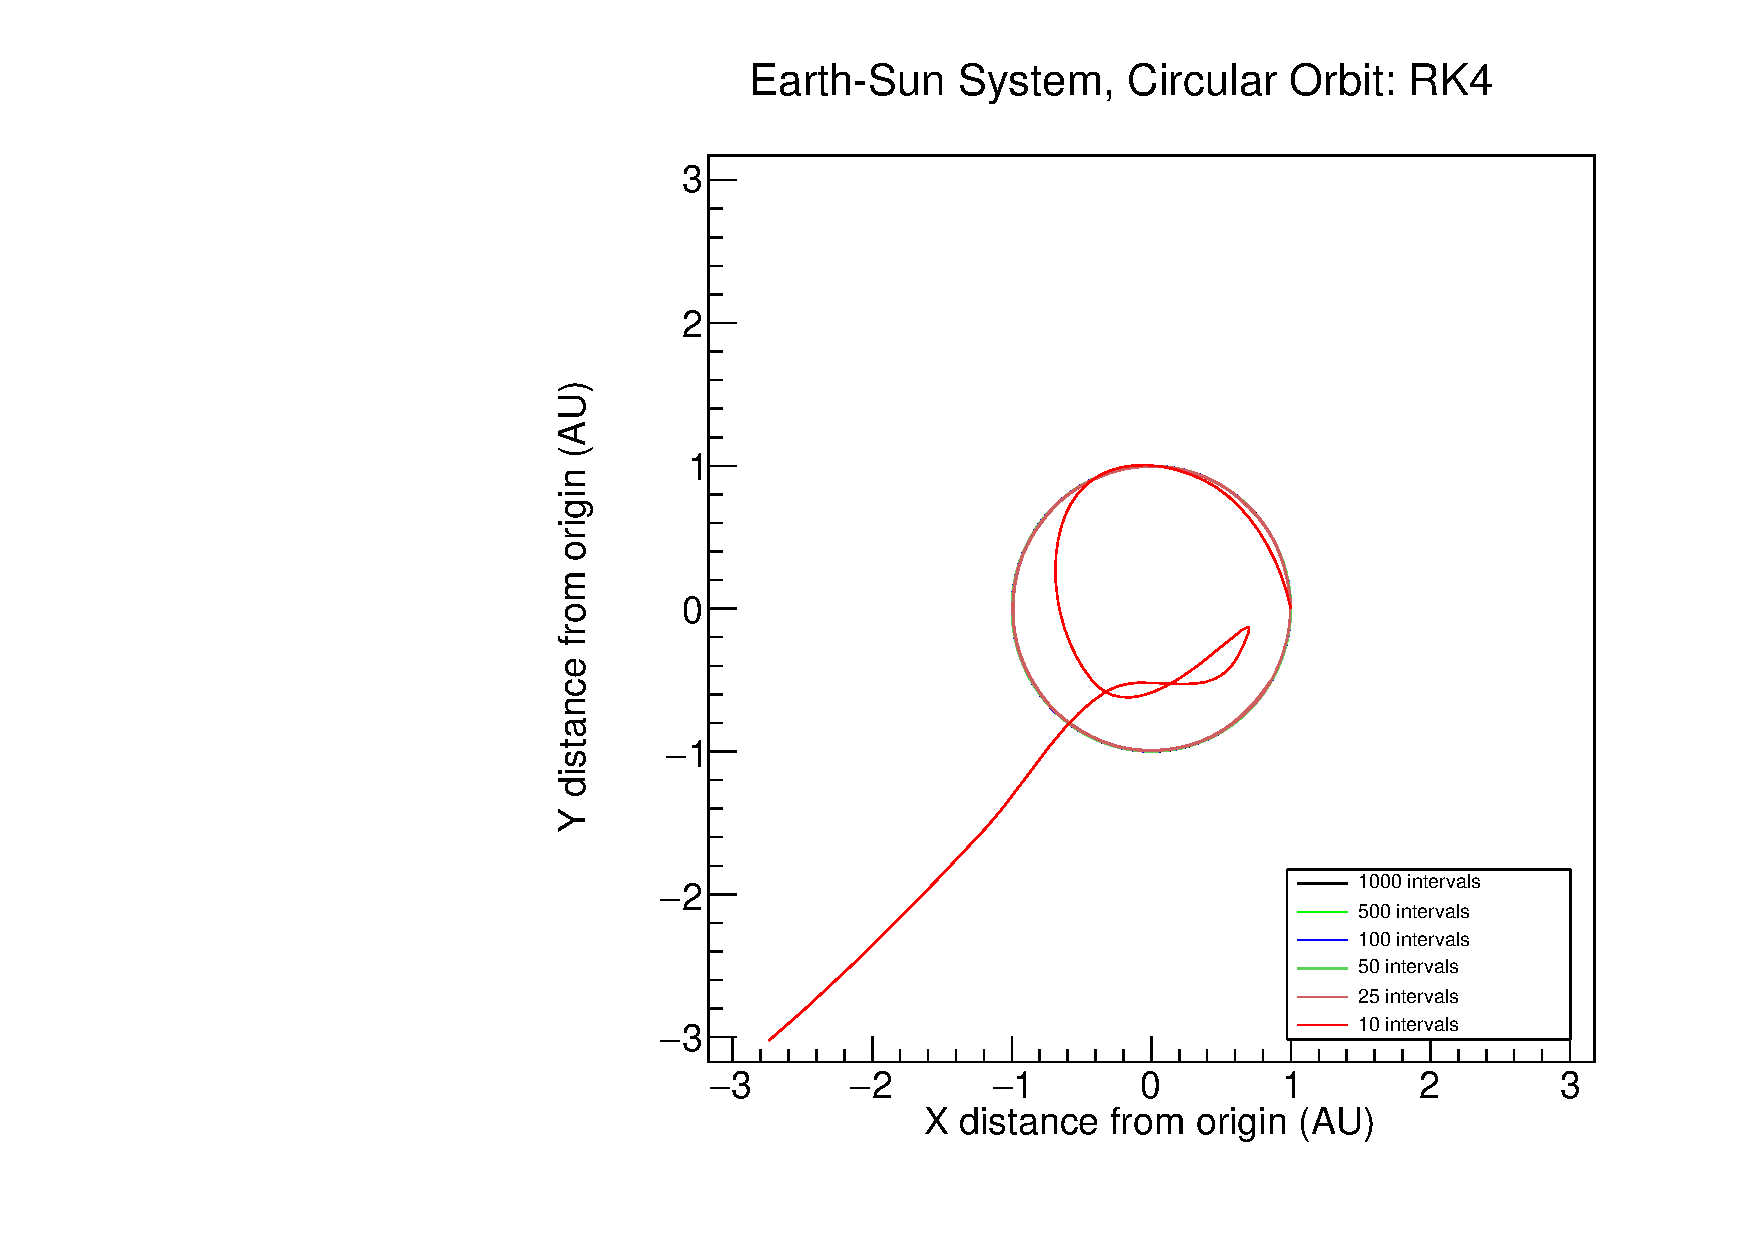
\includegraphics[width=0.5\textwidth]{ESRK4_position.pdf}
  \caption{Plot of Earth's position in Earth-Sun system for different numbers of time steps over 1.9 years using the RK4 algorithm.}
  \label{fig:ESRK4_position}
 \end{SCfigure}

  \begin{SCfigure}
 \centering
   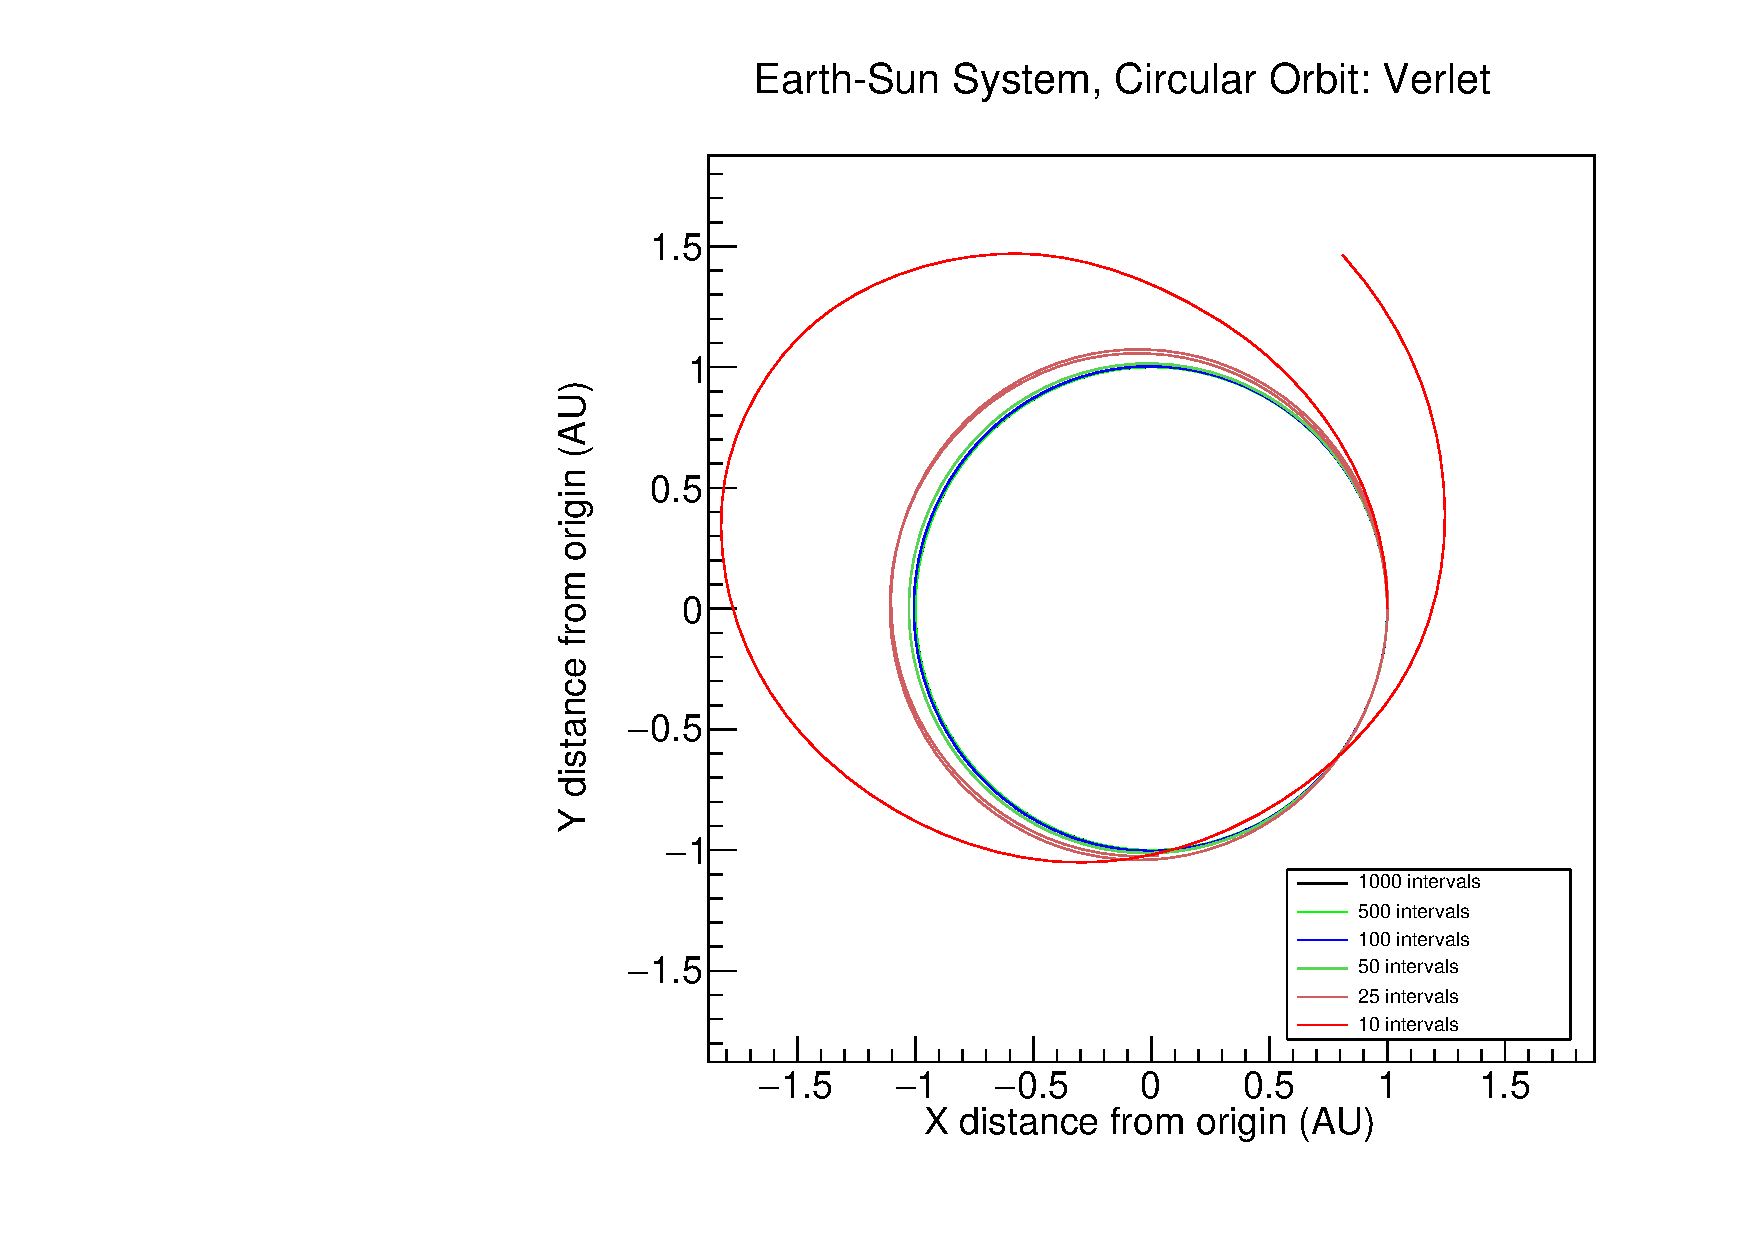
\includegraphics[width=0.5\textwidth]{ESVerlet_position.pdf}
  \caption{Plot of Earth's position in Earth-Sun system for different numbers of time steps over 1.9 years using the Verlet algorithm.}
  \label{fig:ESVerlet_position}
 \end{SCfigure}


\subsection{Escape Velocity}

 \begin{SCfigure}
 \centering
   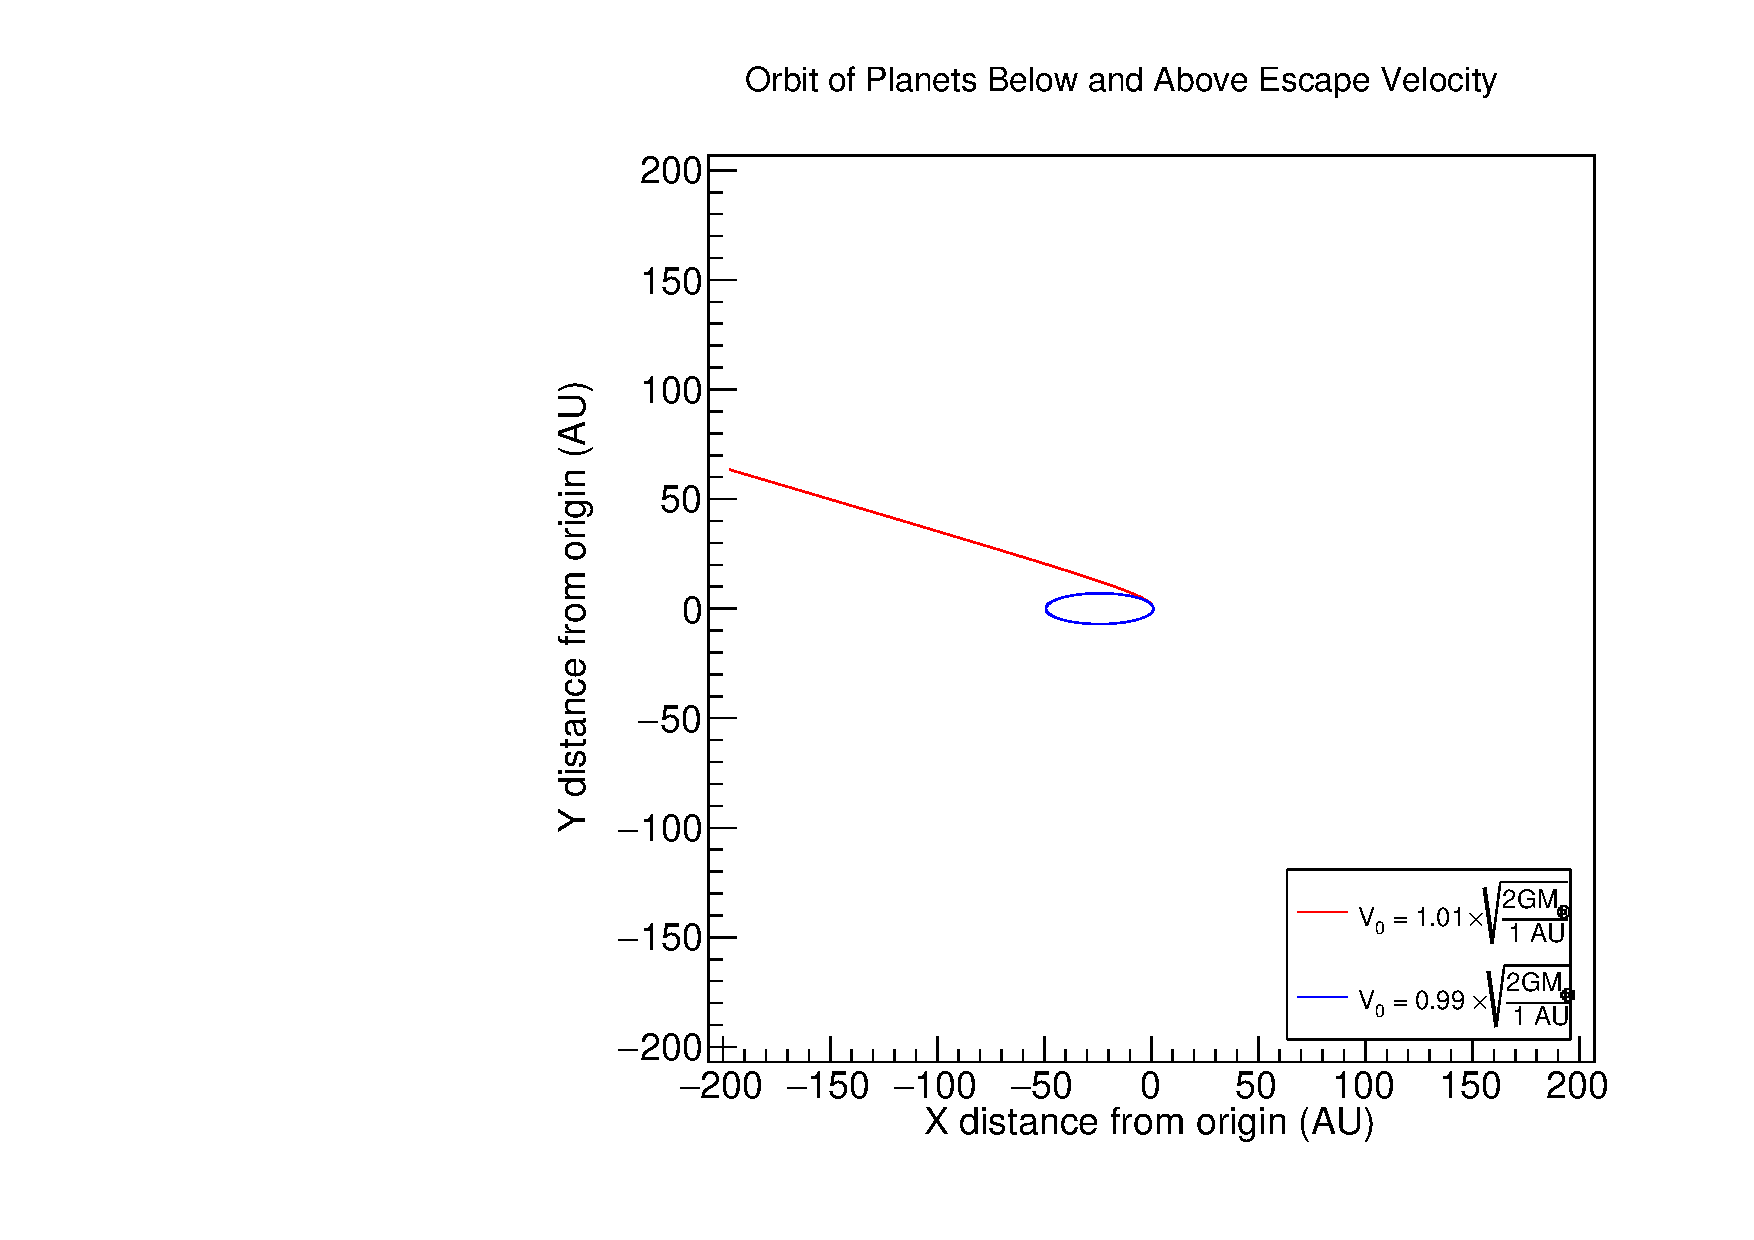
\includegraphics[width=0.5\textwidth]{Escape_plot.pdf}
  \caption{Plot of planet with starting position of 1 AU and starting mass of one Earth mass with initial velocity just above and below escape velocity. Orbital period found by trial and error to be 126 years for the planet just below escape velocity. 20000 time steps were used for accurate orbit modeling.}
  \label{fig:Escape}
 \end{SCfigure}

\subsection{Three Body System: Stationary Sun}

\begin{SCfigure}
 \centering
   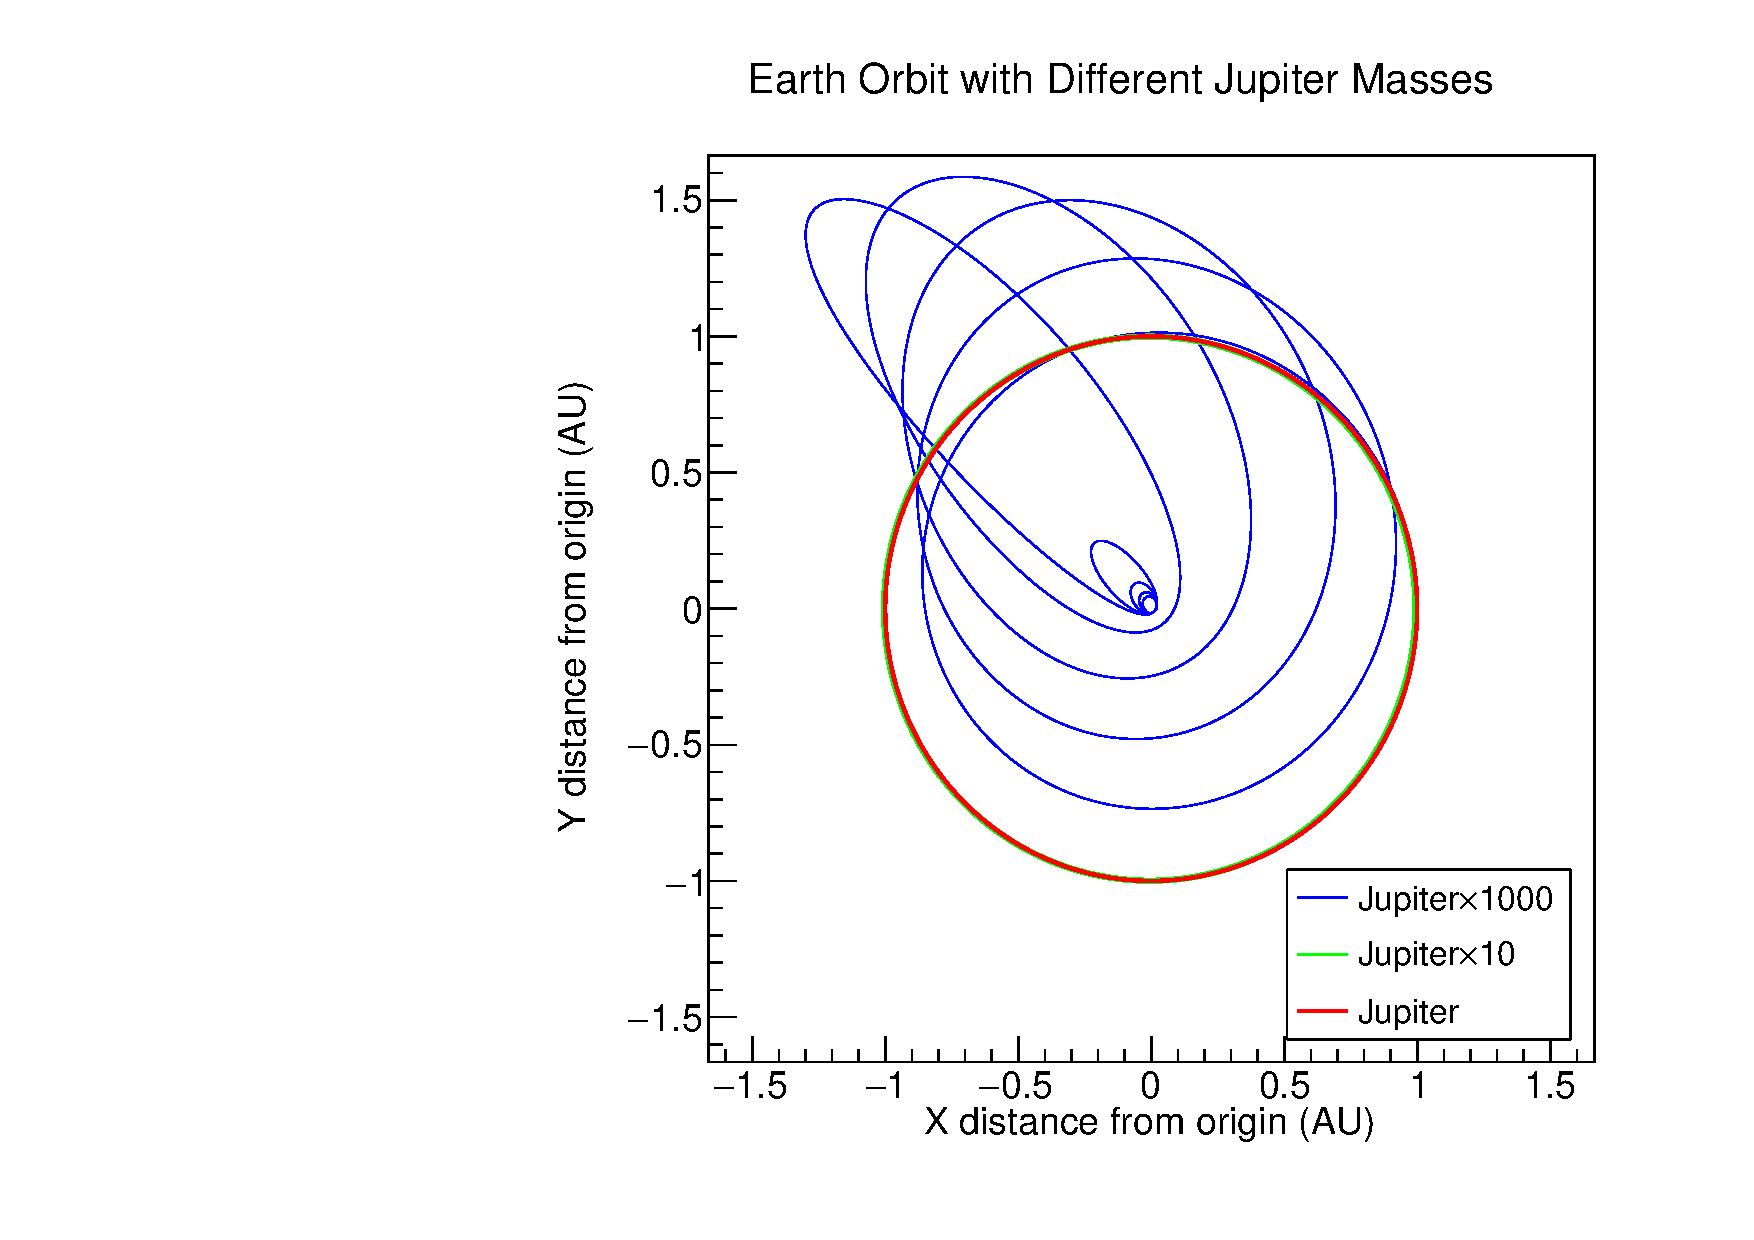
\includegraphics[width=0.5\textwidth]{ESJFRK4_Earths.pdf}
  \caption{Plot of the position of earth in three body system with stationary sun and different Jupiter masses. Used a time length of 13 years with 13000 time steps with the RK4 algorithm.}
  \label{fig:ESJFRK4_Earths}
 \end{SCfigure}

 \begin{SCfigure}
 \centering
   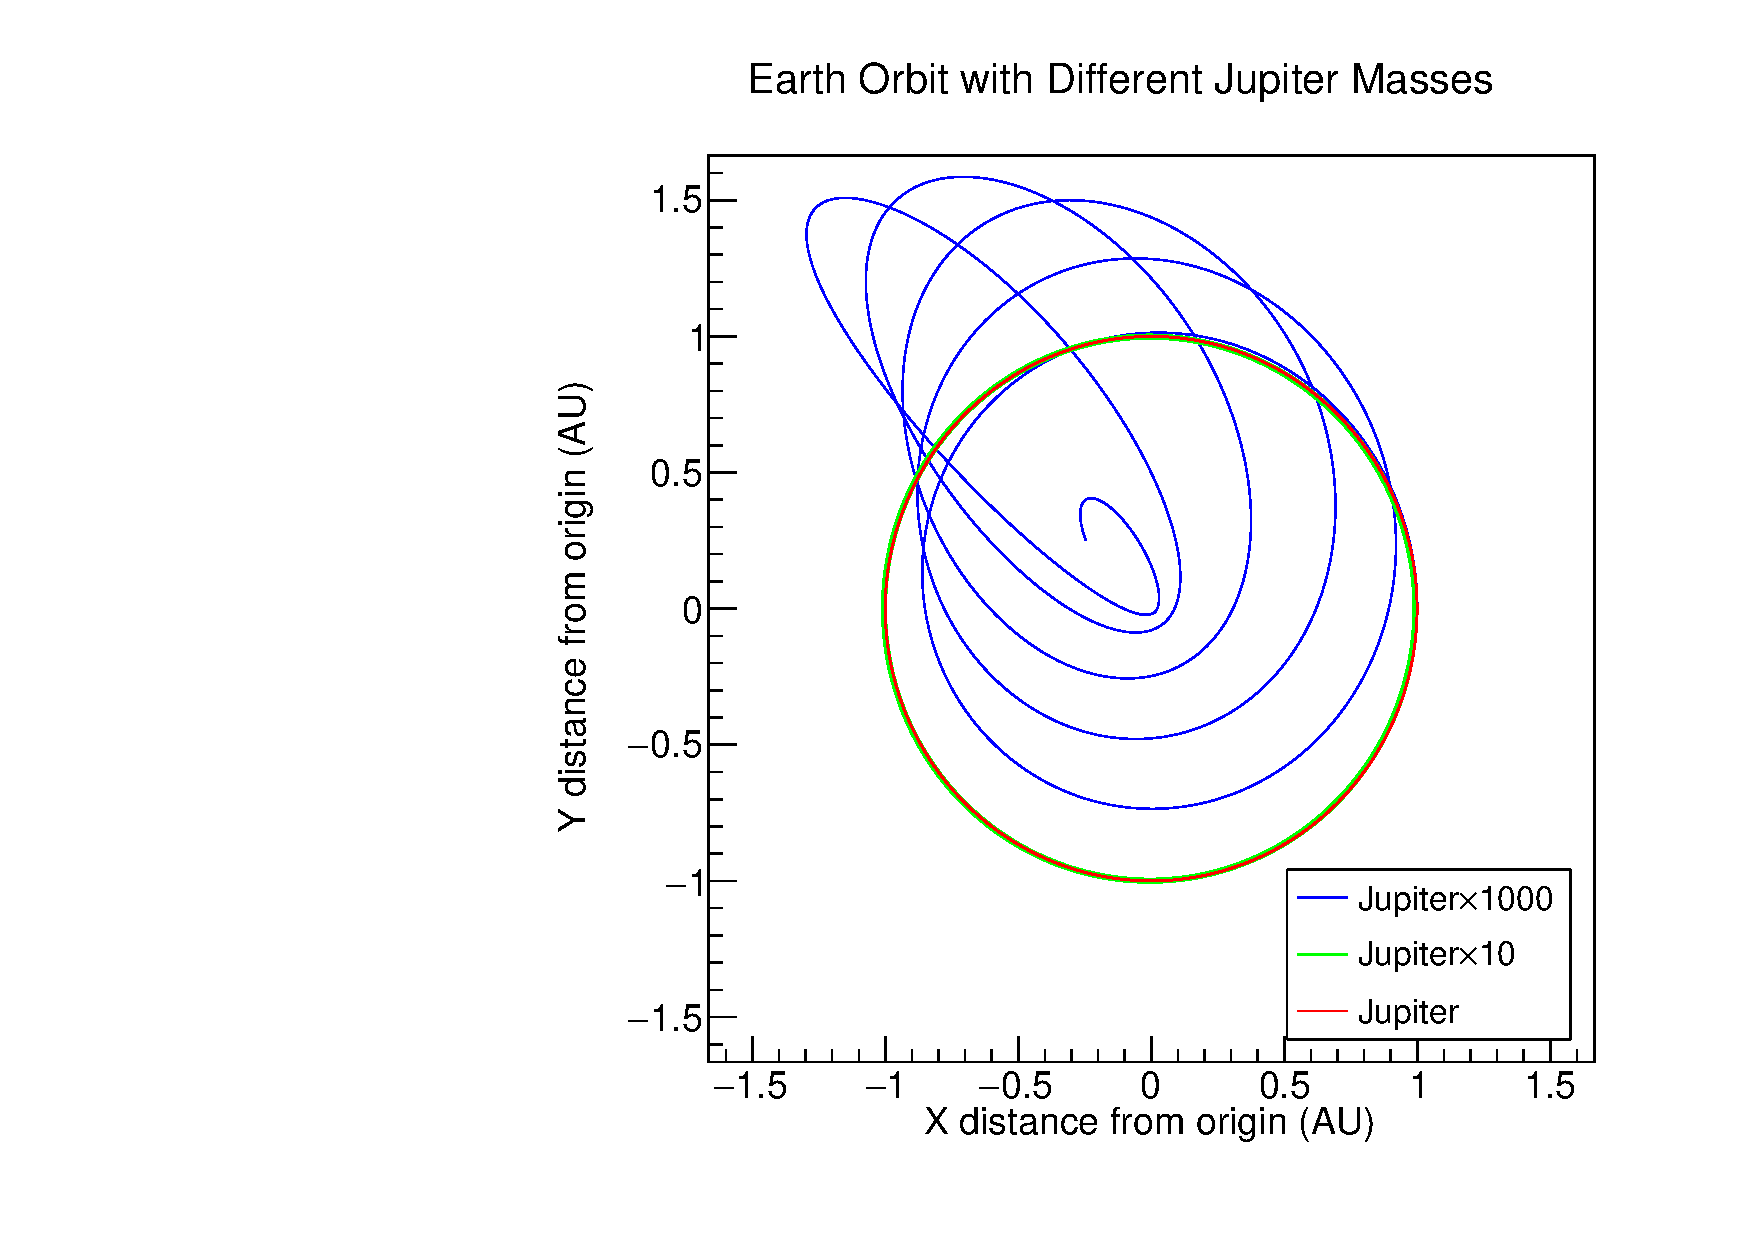
\includegraphics[width=0.5\textwidth]{ESJFVerlet_Earths.pdf}
  \caption{Plot of the position of earth in three body system with stationary sun and different Jupiter masses. Used a time length of 13 years with 13000 time steps with the Verlet algorithm.}
  \label{fig:ESJFVerlet_Earths}
 \end{SCfigure}


\subsection{Onwards: 3 Dynamic Bodies and All Major Bodies}

\section{Conclusion}\label{sec:conclude}


\appendix
\addtocontents{toc}{\protect\contentsline{chapter}{Appendix:}{}}
\chapter{Earth-Sun Plots}\label{app:esplots}

\begin{figure}[H]
 \centering
   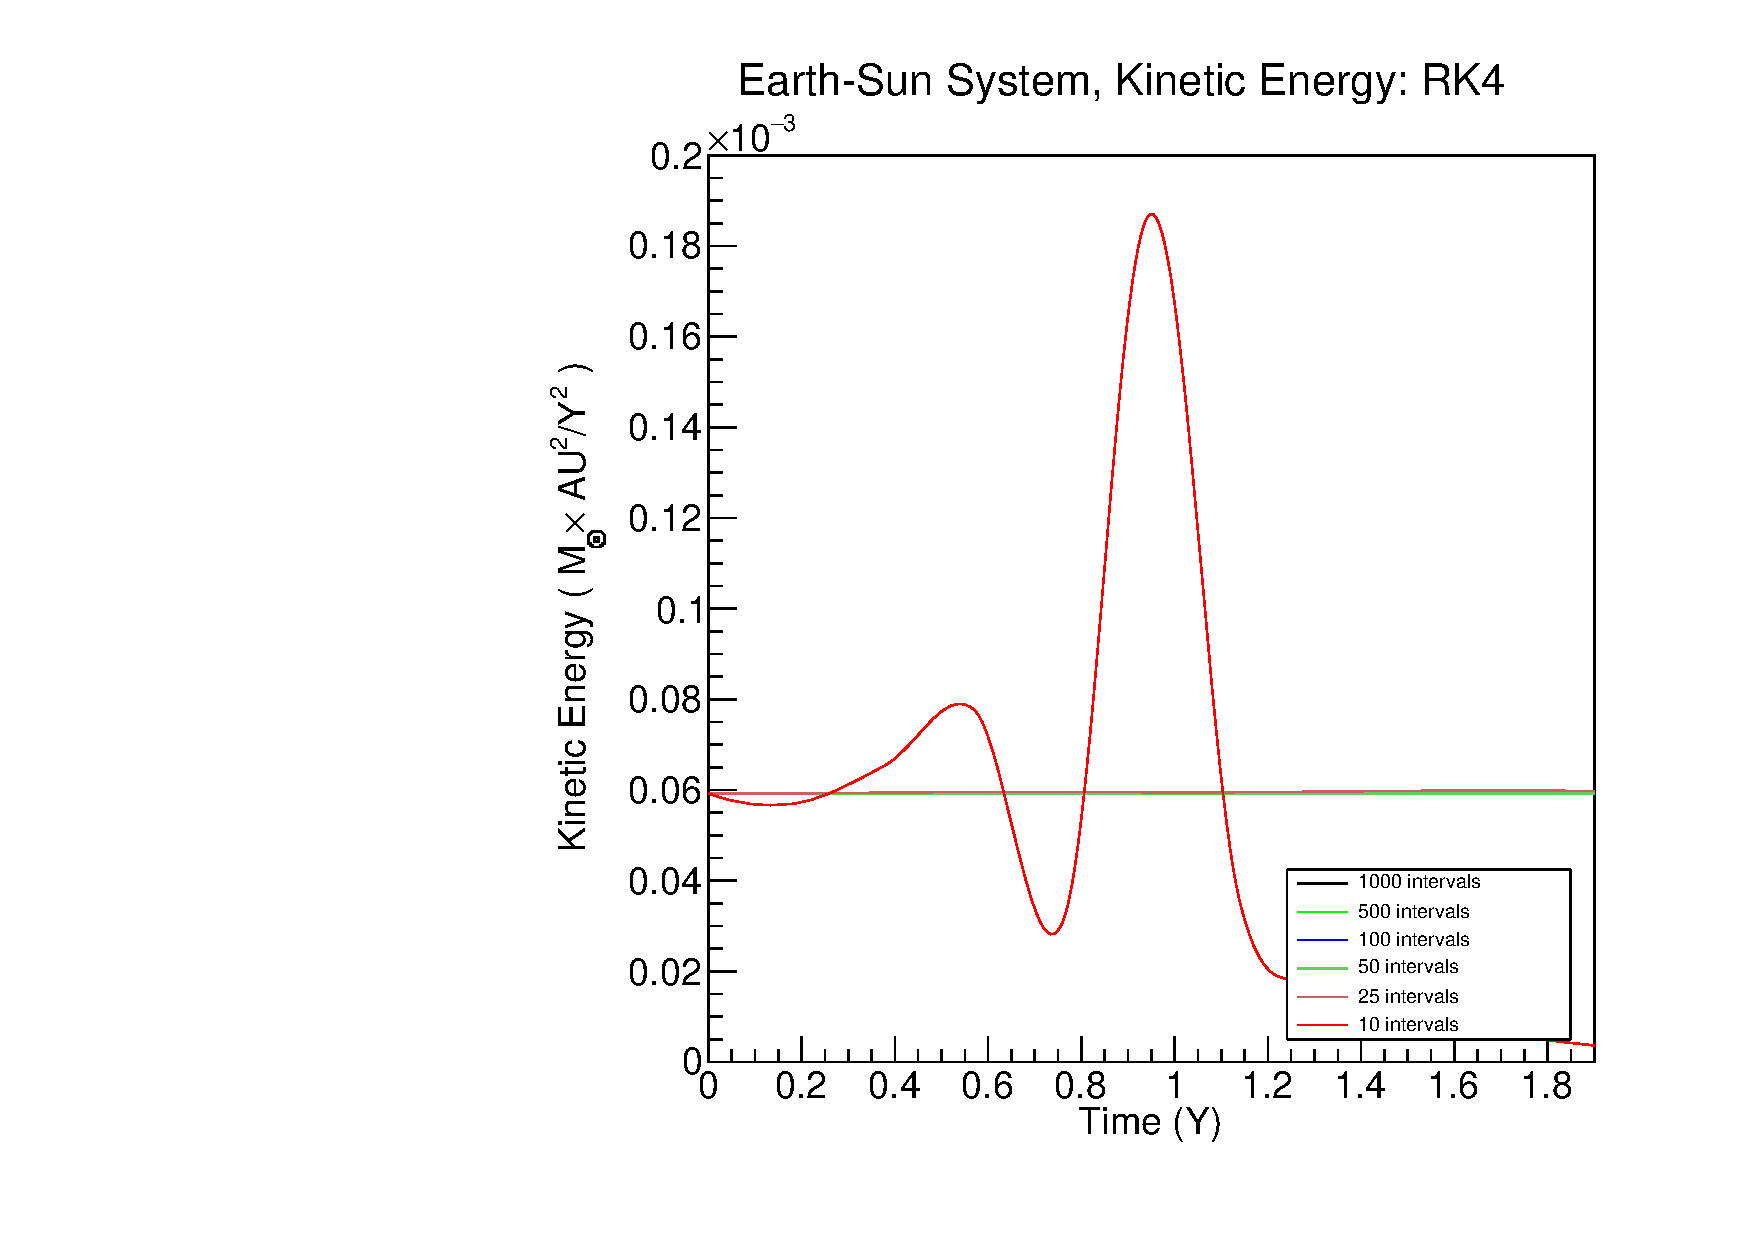
\includegraphics[width=0.5\textwidth]{ESRK4_ke.pdf}
  \caption{Plot of Earth-Sun system kinetic energy for different numbers of time steps over 1.9 years using the RK4 algorithm.}
  \label{fig:ESRK4_ke}
 \end{figure}
 
   \begin{figure}[H]
 \centering
   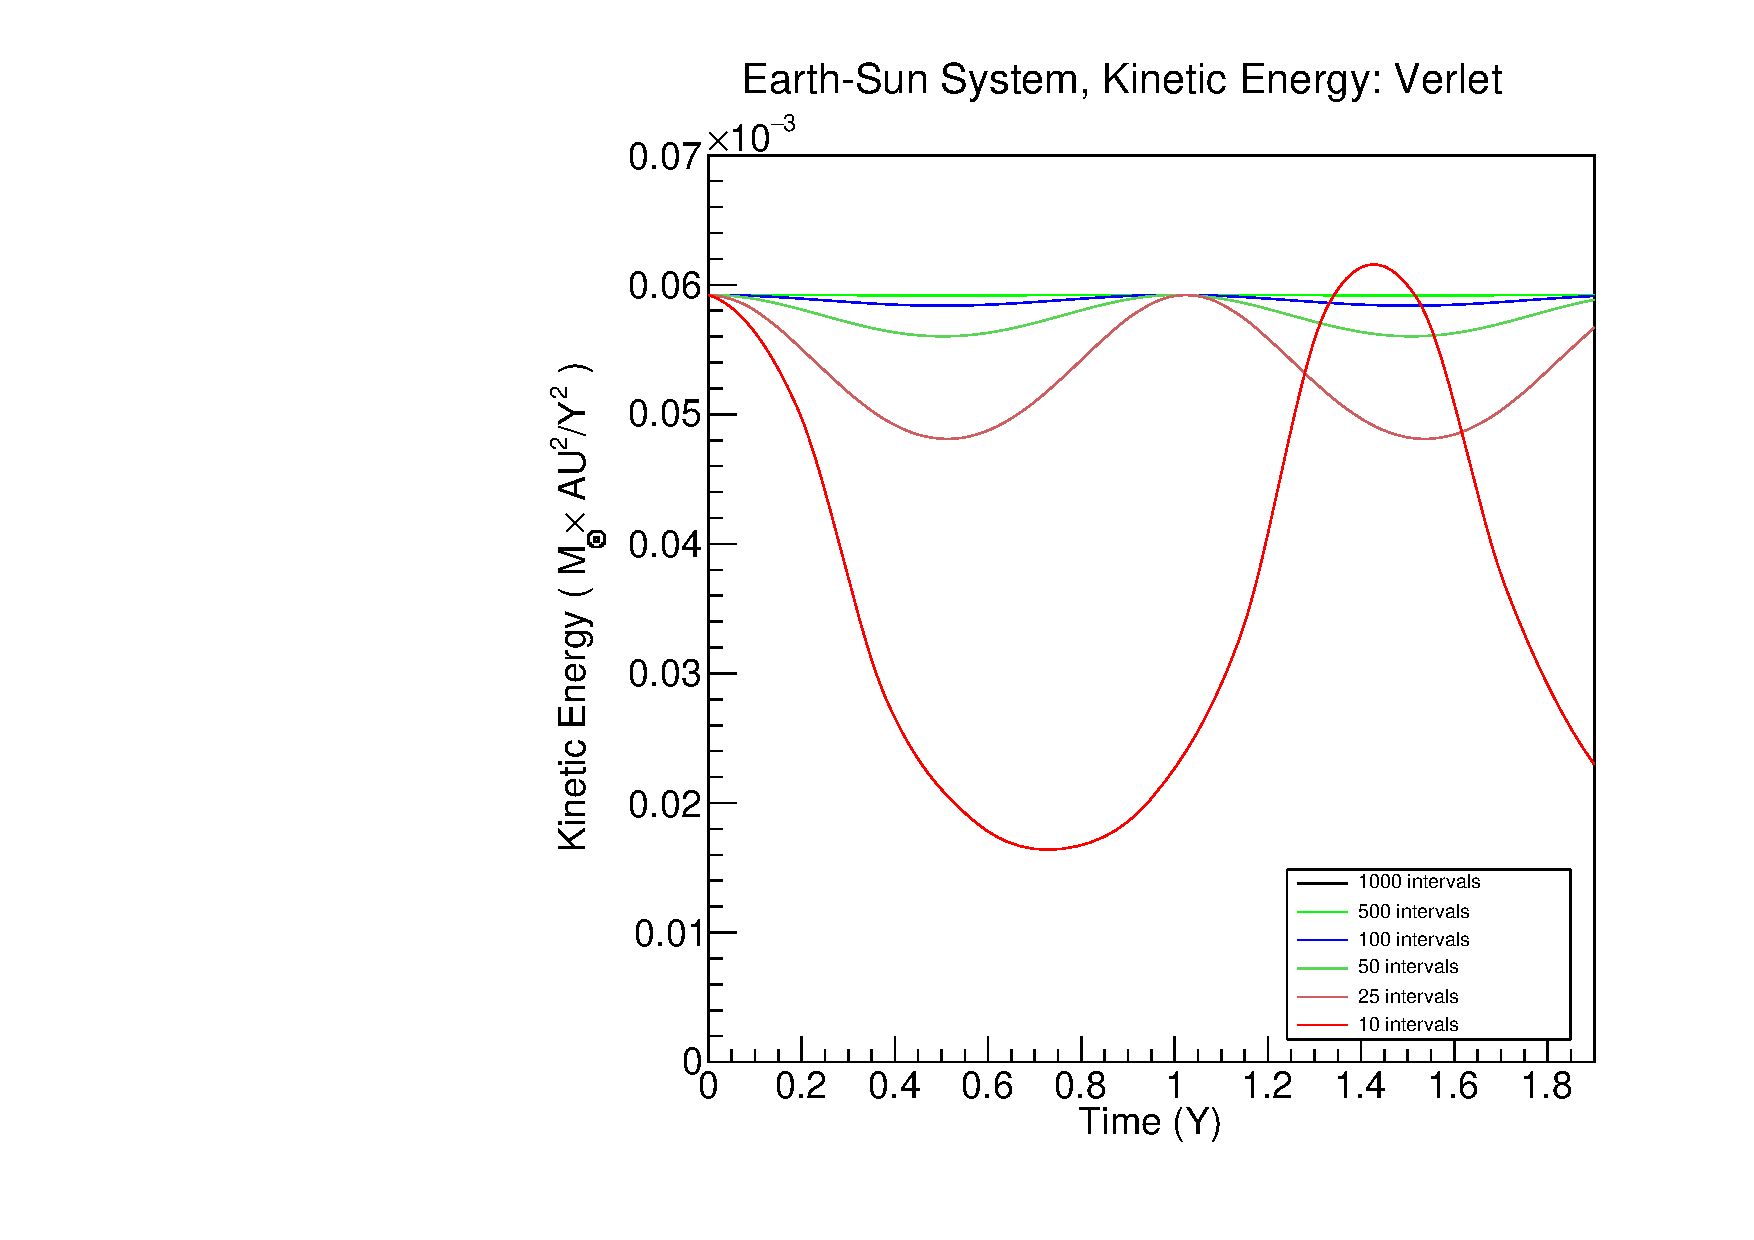
\includegraphics[width=0.5\textwidth]{ESVerlet_ke.pdf}
  \caption{Plot of Earth-Sun system kinetic energy for different numbers of time steps over 1.9 years using the Verlet algorithm.}
  \label{fig:ESVerlet_ke}
 \end{figure}


\begin{figure}[H]
 \centering
   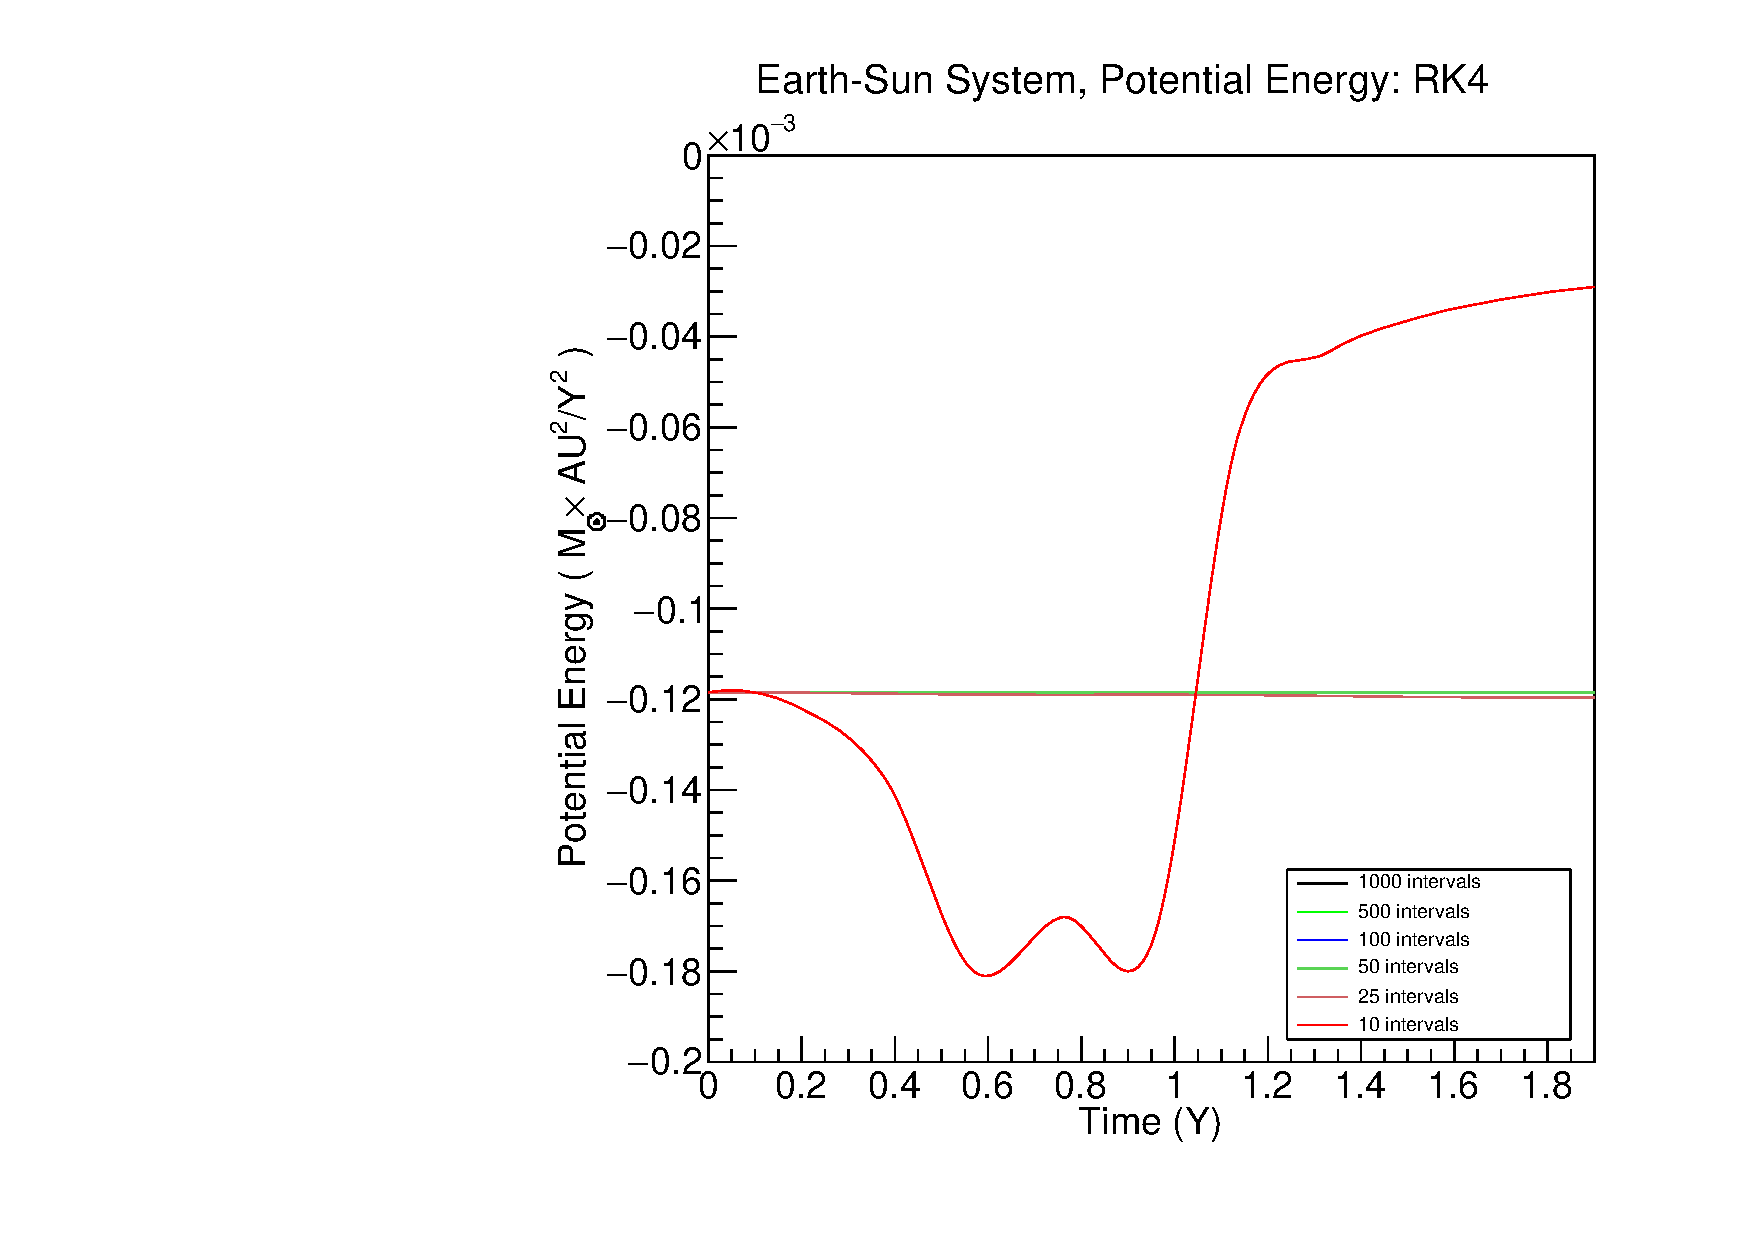
\includegraphics[width=0.5\textwidth]{ESRK4_pe.pdf}
  \caption{Plot of Earth-Sun system potential energy for different numbers of time steps over 1.9 years using the RK4 algorithm.}
  \label{fig:ESRK4_pe}
 \end{figure}

 \begin{figure}[H]
 \centering
   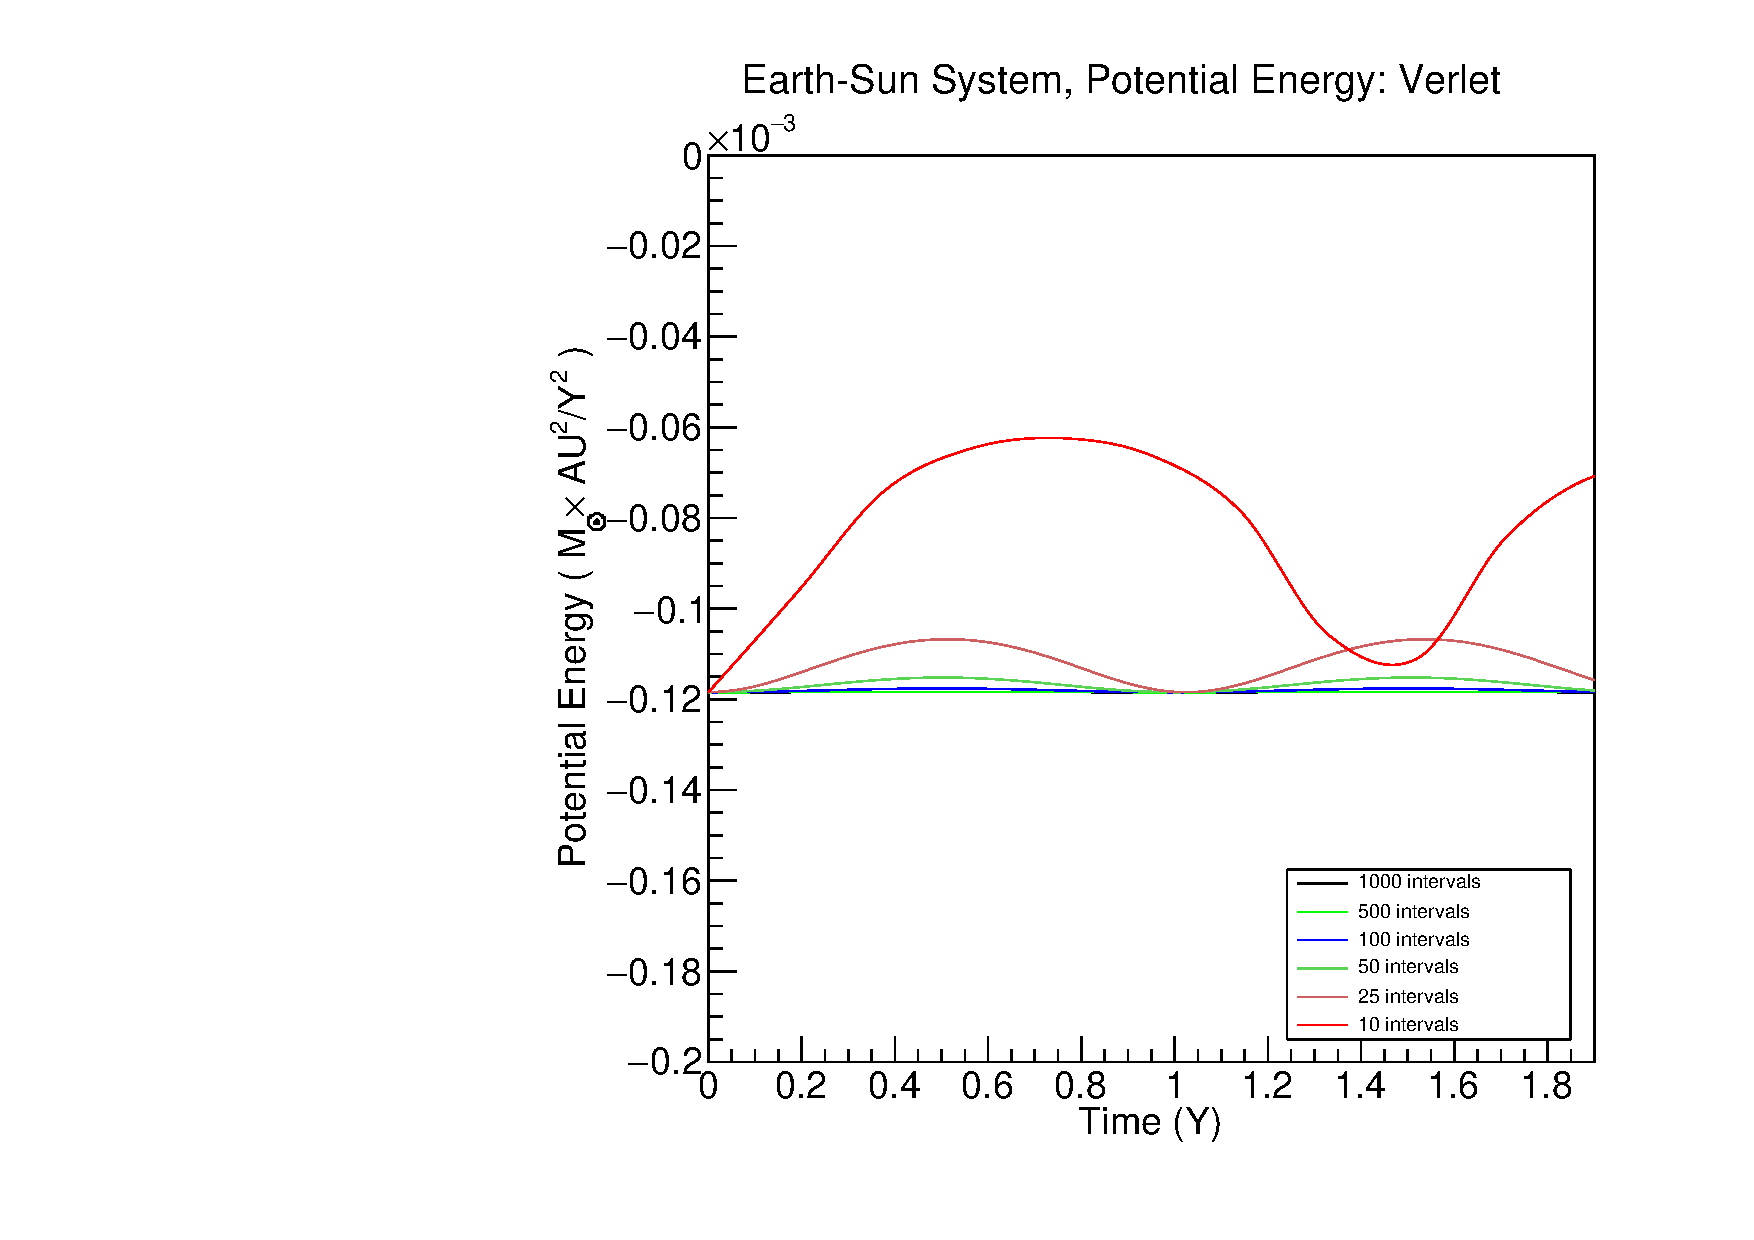
\includegraphics[width=0.5\textwidth]{ESVerlet_pe.pdf}
  \caption{Plot of Earth-Sun system potential energy for different numbers of time steps over 1.9 years using the Verlet algorithm.}
  \label{fig:ESVerlet_pe}
 \end{figure}

\begin{figure}[H]
 \centering
   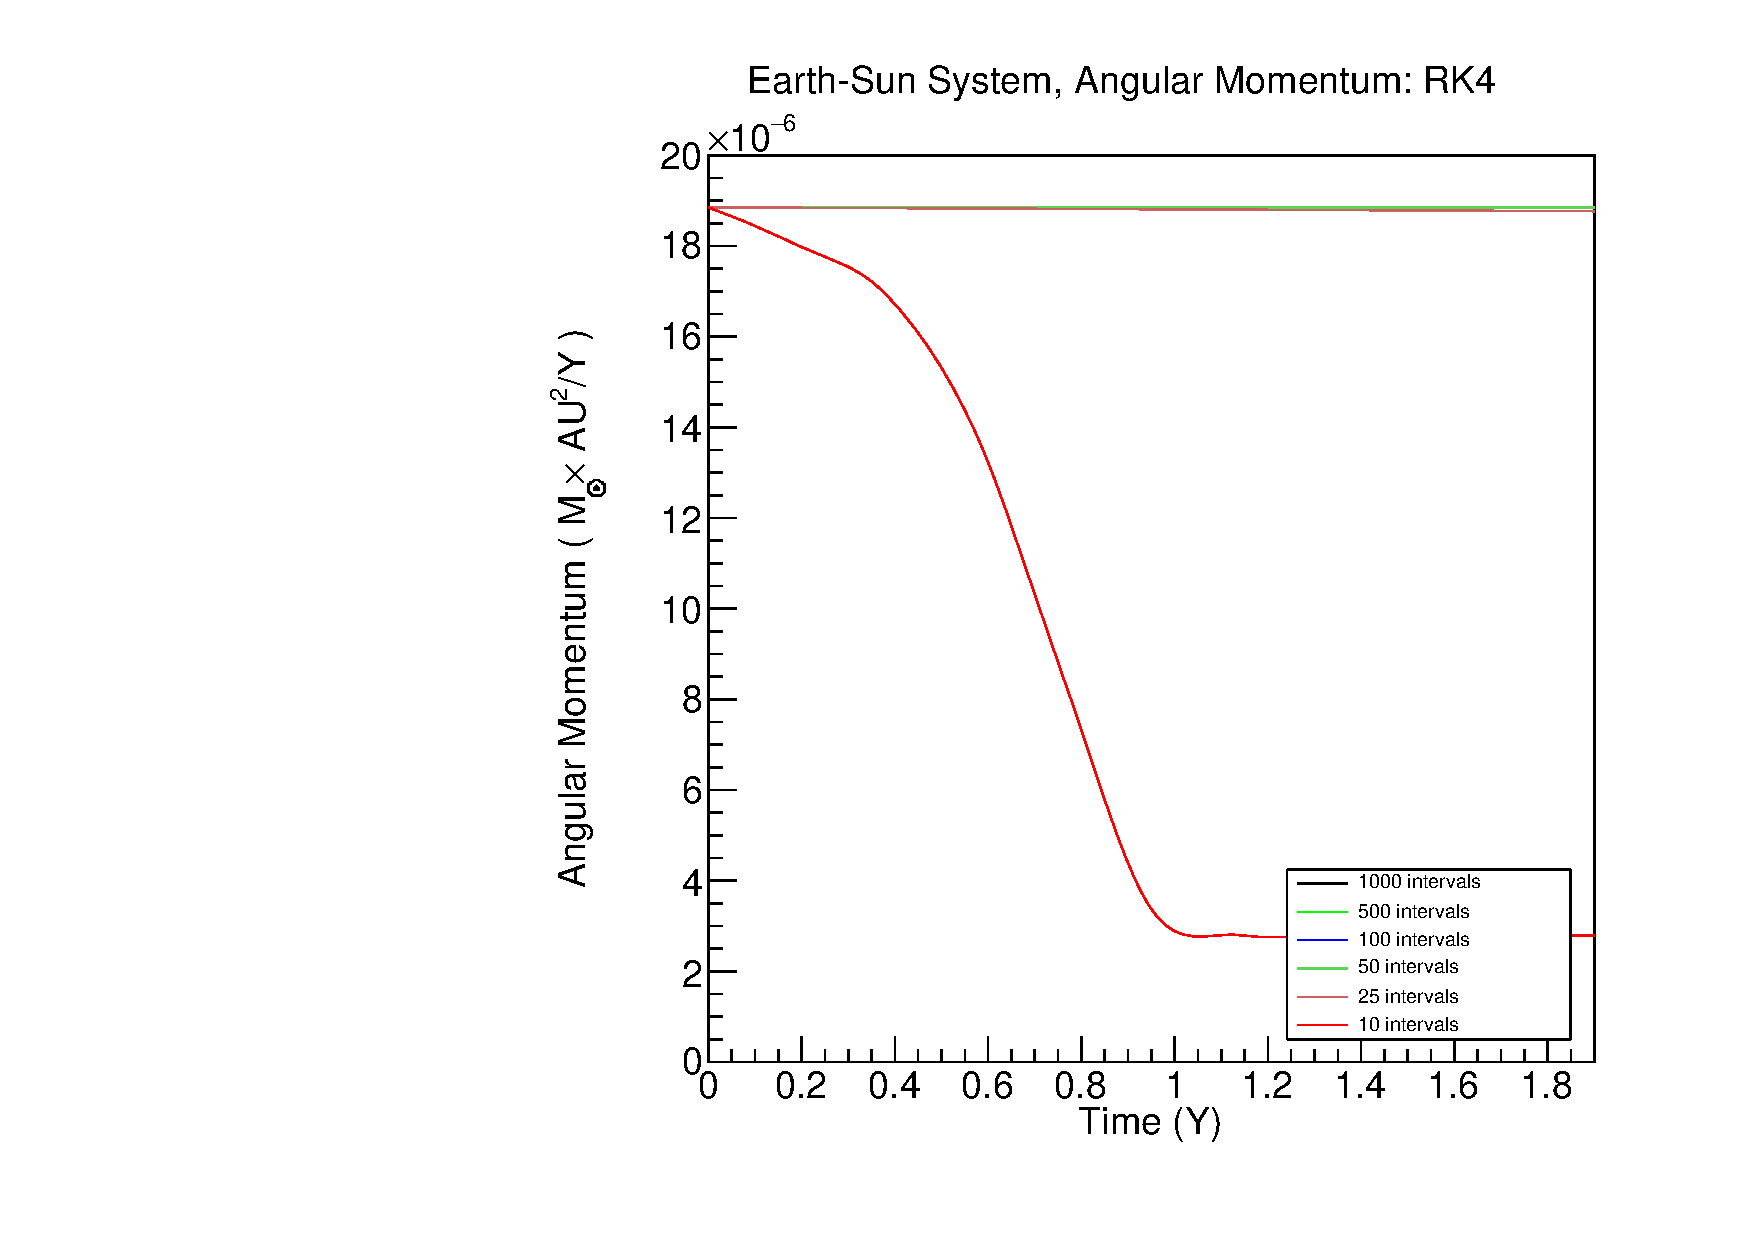
\includegraphics[width=0.5\textwidth]{ESRK4_l.pdf}
  \caption{Plot of Earth-Sun system angular momentum for different numbers of time steps over 1.9 years using the RK4 algorithm.}
  \label{fig:ESRK4_l}
 \end{figure}



\begin{figure}[H]
 \centering
   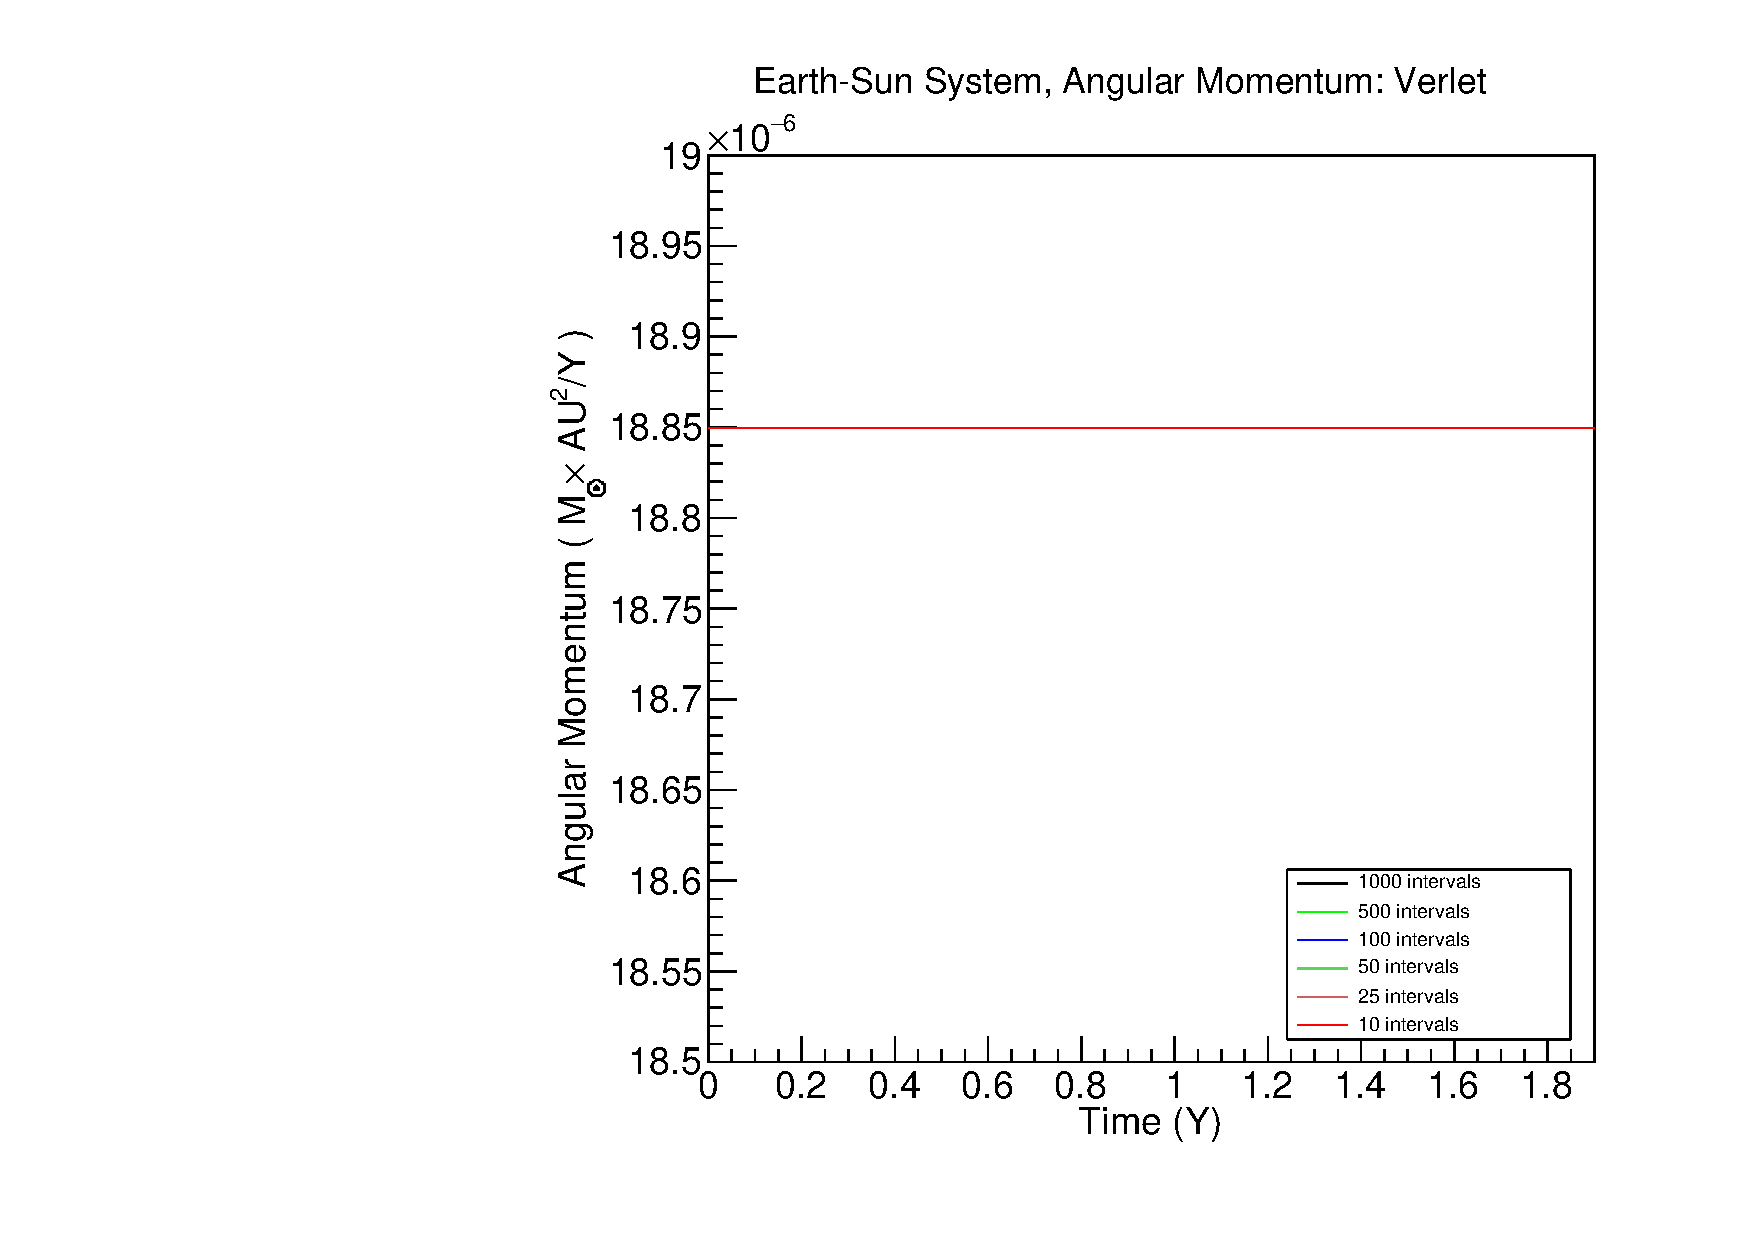
\includegraphics[width=0.5\textwidth]{ESVerlet_l.pdf}
  \caption{Plot of Earth-Sun system angular momentum for different numbers of time steps over 1.9 years using the Verlet algorithm.}
  \label{fig:ESVerlet_l}
 \end{figure}
 
 \chapter{Three Body System: Stationary Sun Plots}\label{app:3bsss}
 
 \begin{figure}[H]
 \centering
   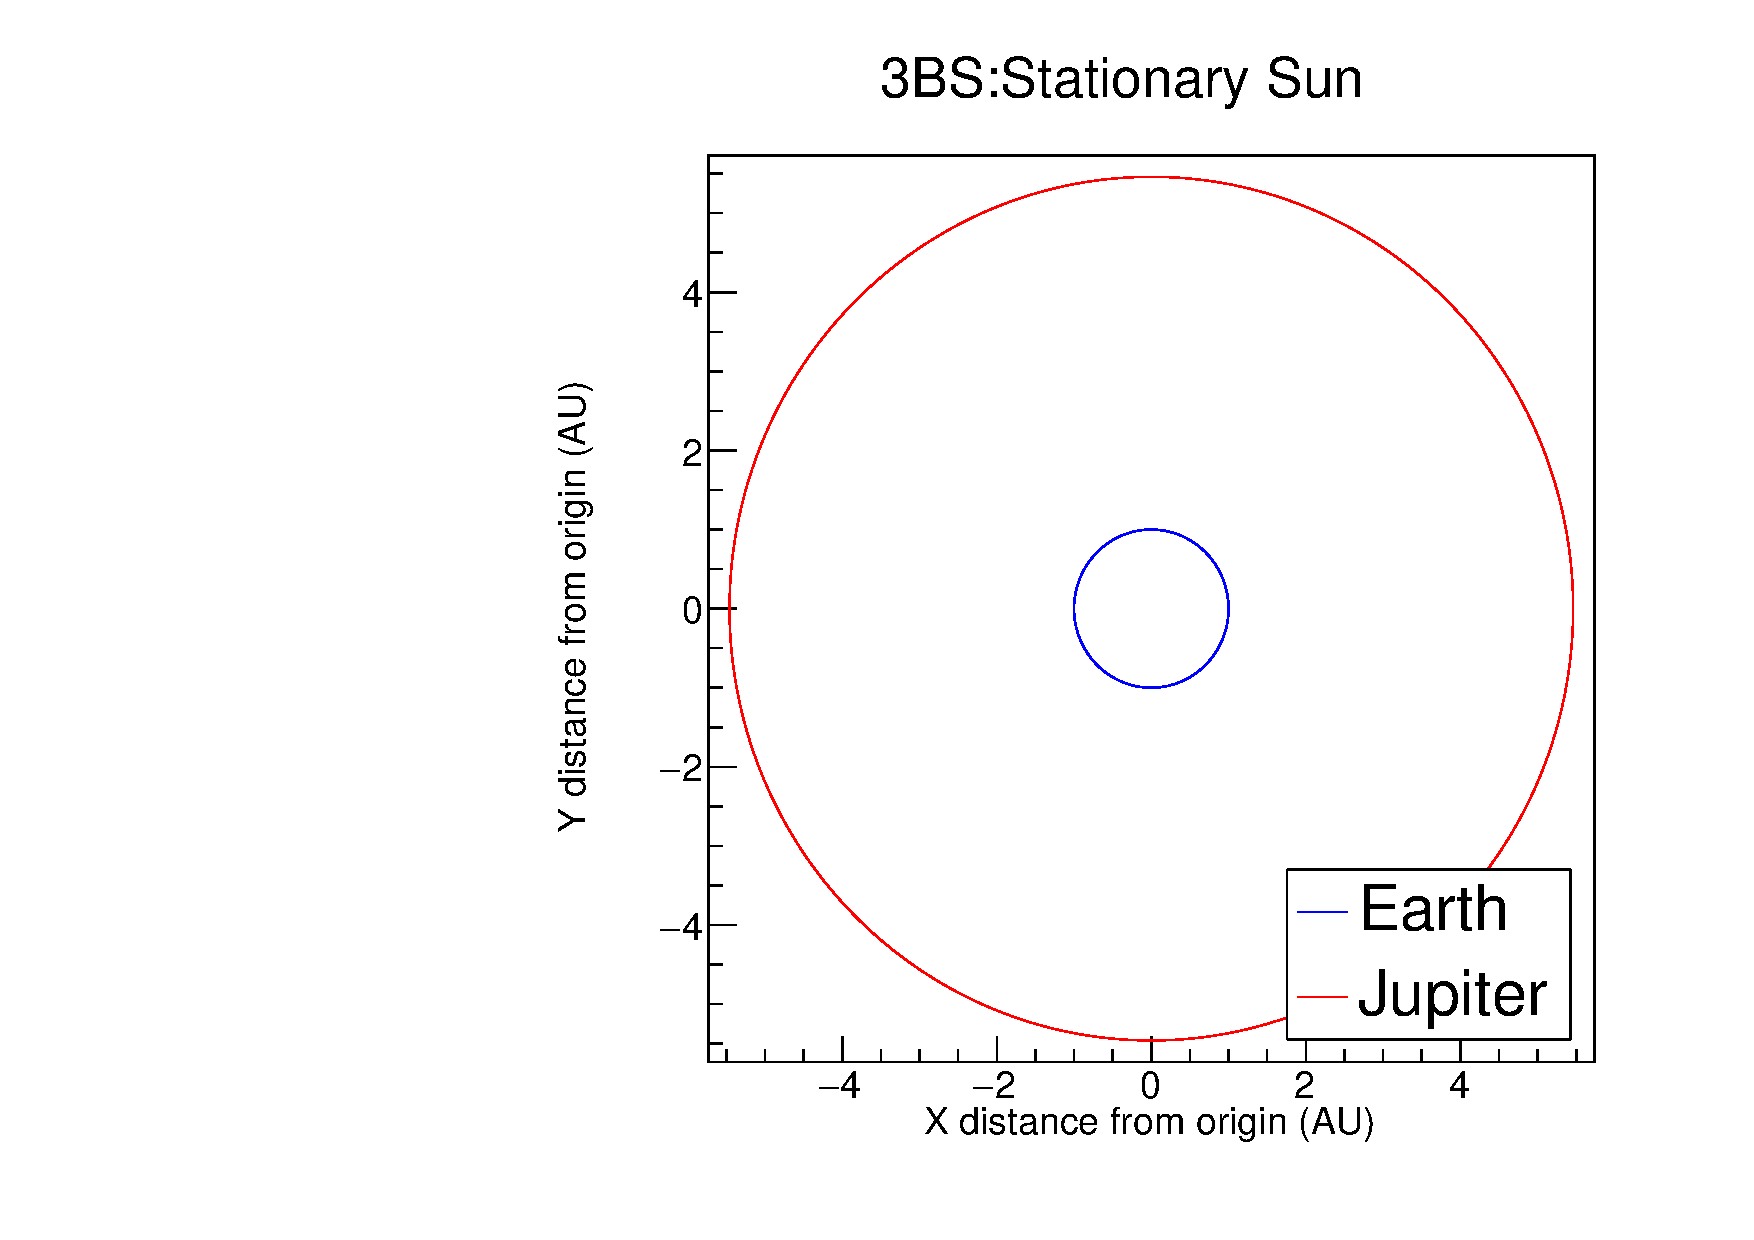
\includegraphics[width=0.5\textwidth]{ESJFRK4_reg.pdf}
  \caption{Plot of 3 body system with Earth, Jupiter, and a stationary sun using regular Jupiter mass. Time interval: 13 years, Time steps: 13000, Algorithm: RK4.}
  \label{fig:ESJFRK4_reg}
 \end{figure}
 
  \begin{figure}[H]
 \centering
   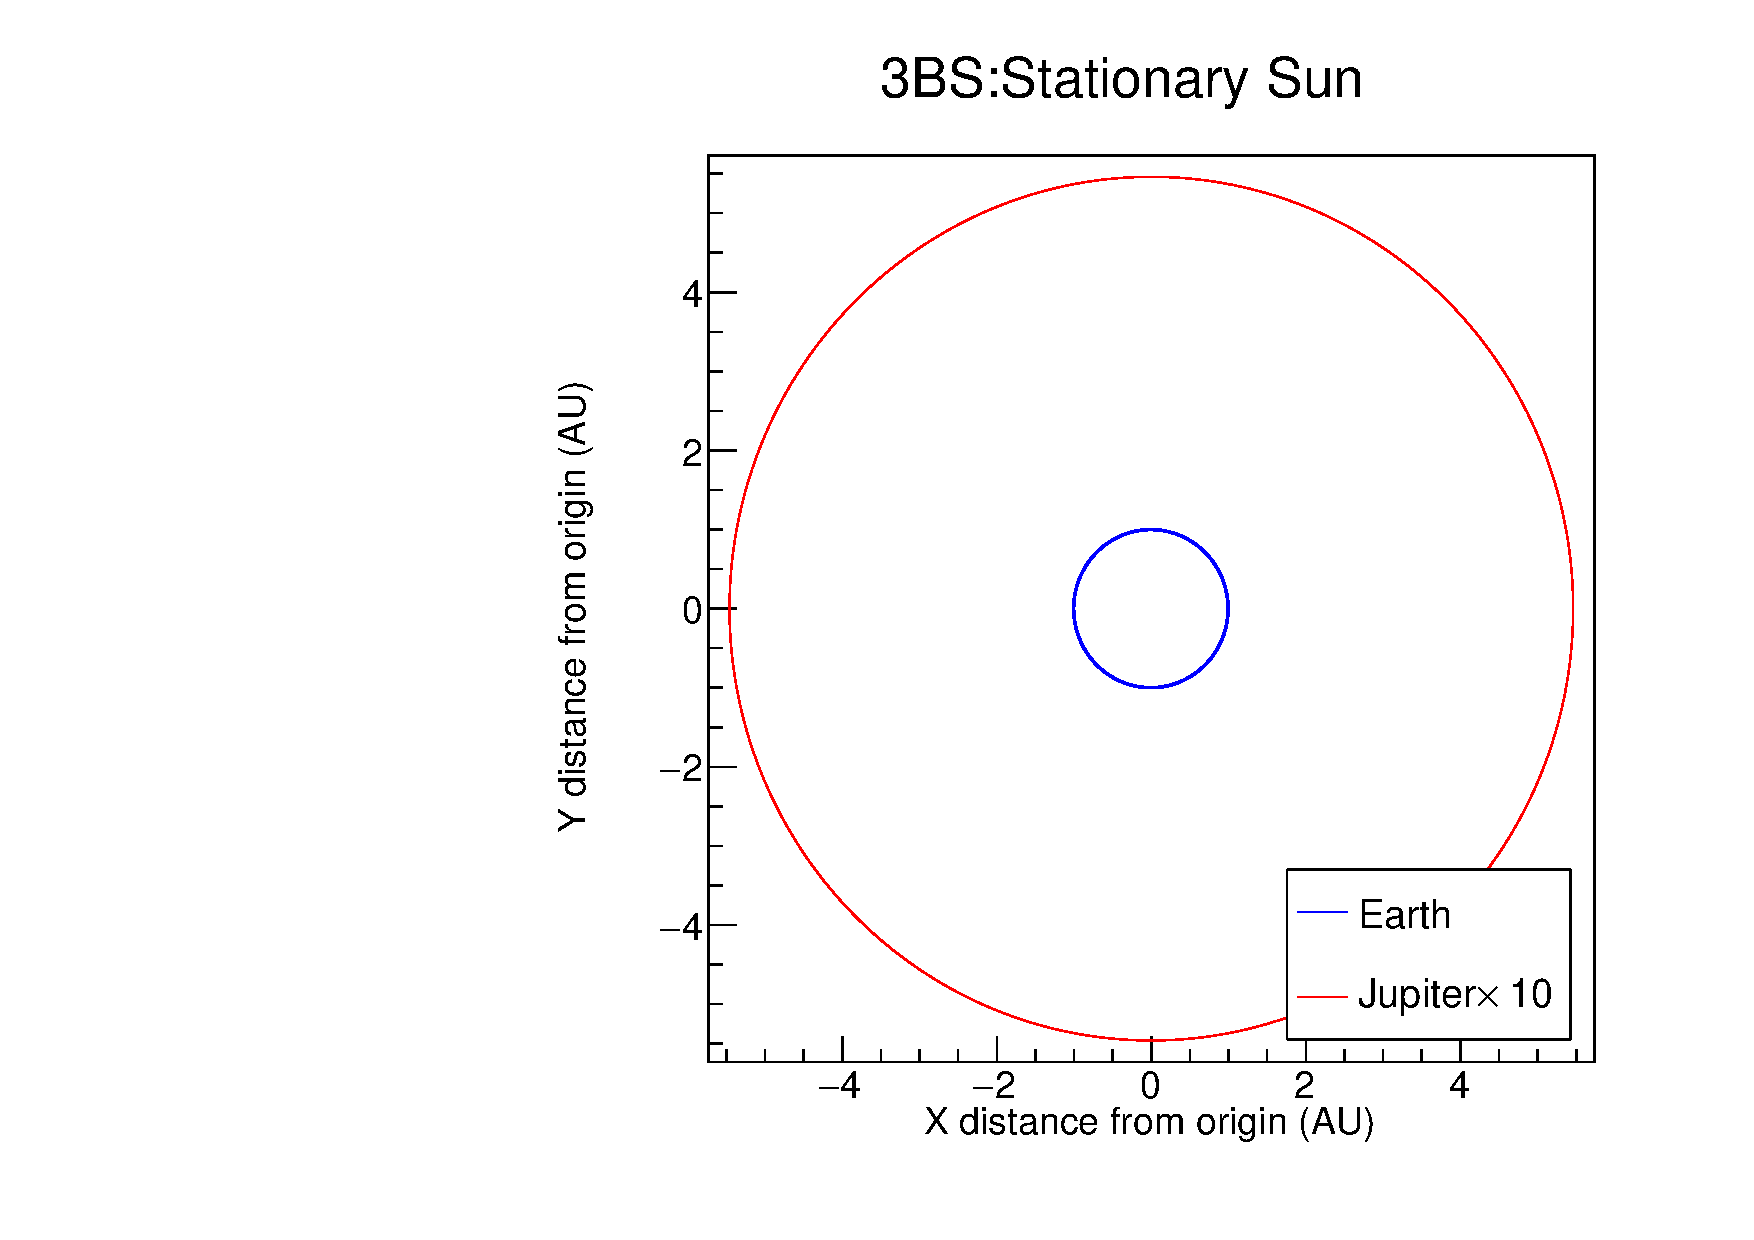
\includegraphics[width=0.5\textwidth]{ESJFRK4_x10.pdf}
  \caption{Plot of 3 body system with Earth, Jupiter, and a stationary sun using $\times 10$ Jupiter mass. Time interval: 13 years, Time steps: 13000, Algorithm: RK4.}
  \label{fig:ESJFRK4_x10}
 \end{figure}
 
  \begin{figure}[H]
 \centering
   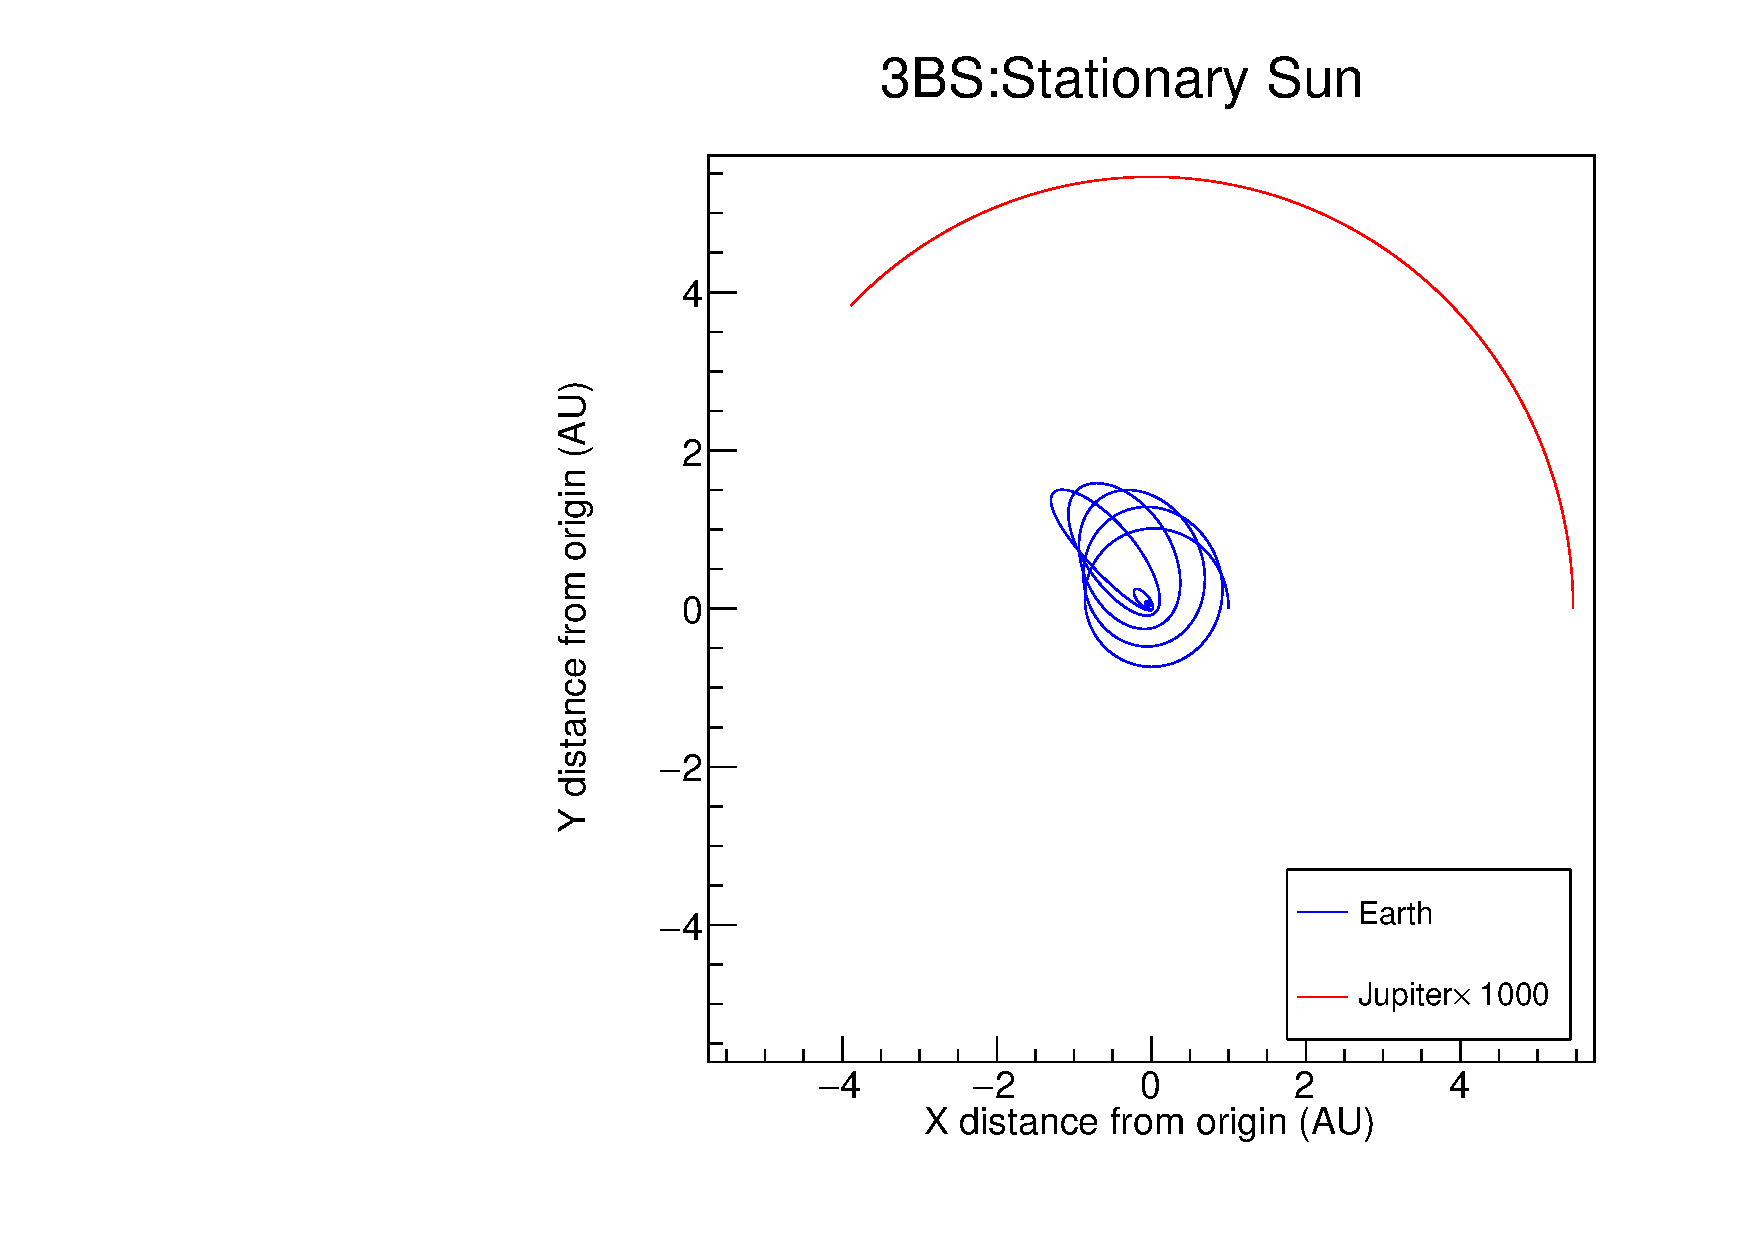
\includegraphics[width=0.5\textwidth]{ESJFRK4_x1000.pdf}
  \caption{Plot of 3 body system with Earth, Jupiter, and a stationary sun using $\times 1000$ Jupiter mass. Used a shorter timespan because this heavy Jupiter causes Earth to ``hit the sun'', then go barreling out many AU so the orbital structure is no longer visible. Time interval: 4.8 years, Time steps: 13000, Algorithm: RK4.}
  \label{fig:ESJFRK4_x1000}
 \end{figure}
 
 \begin{figure}[H]
 \centering
   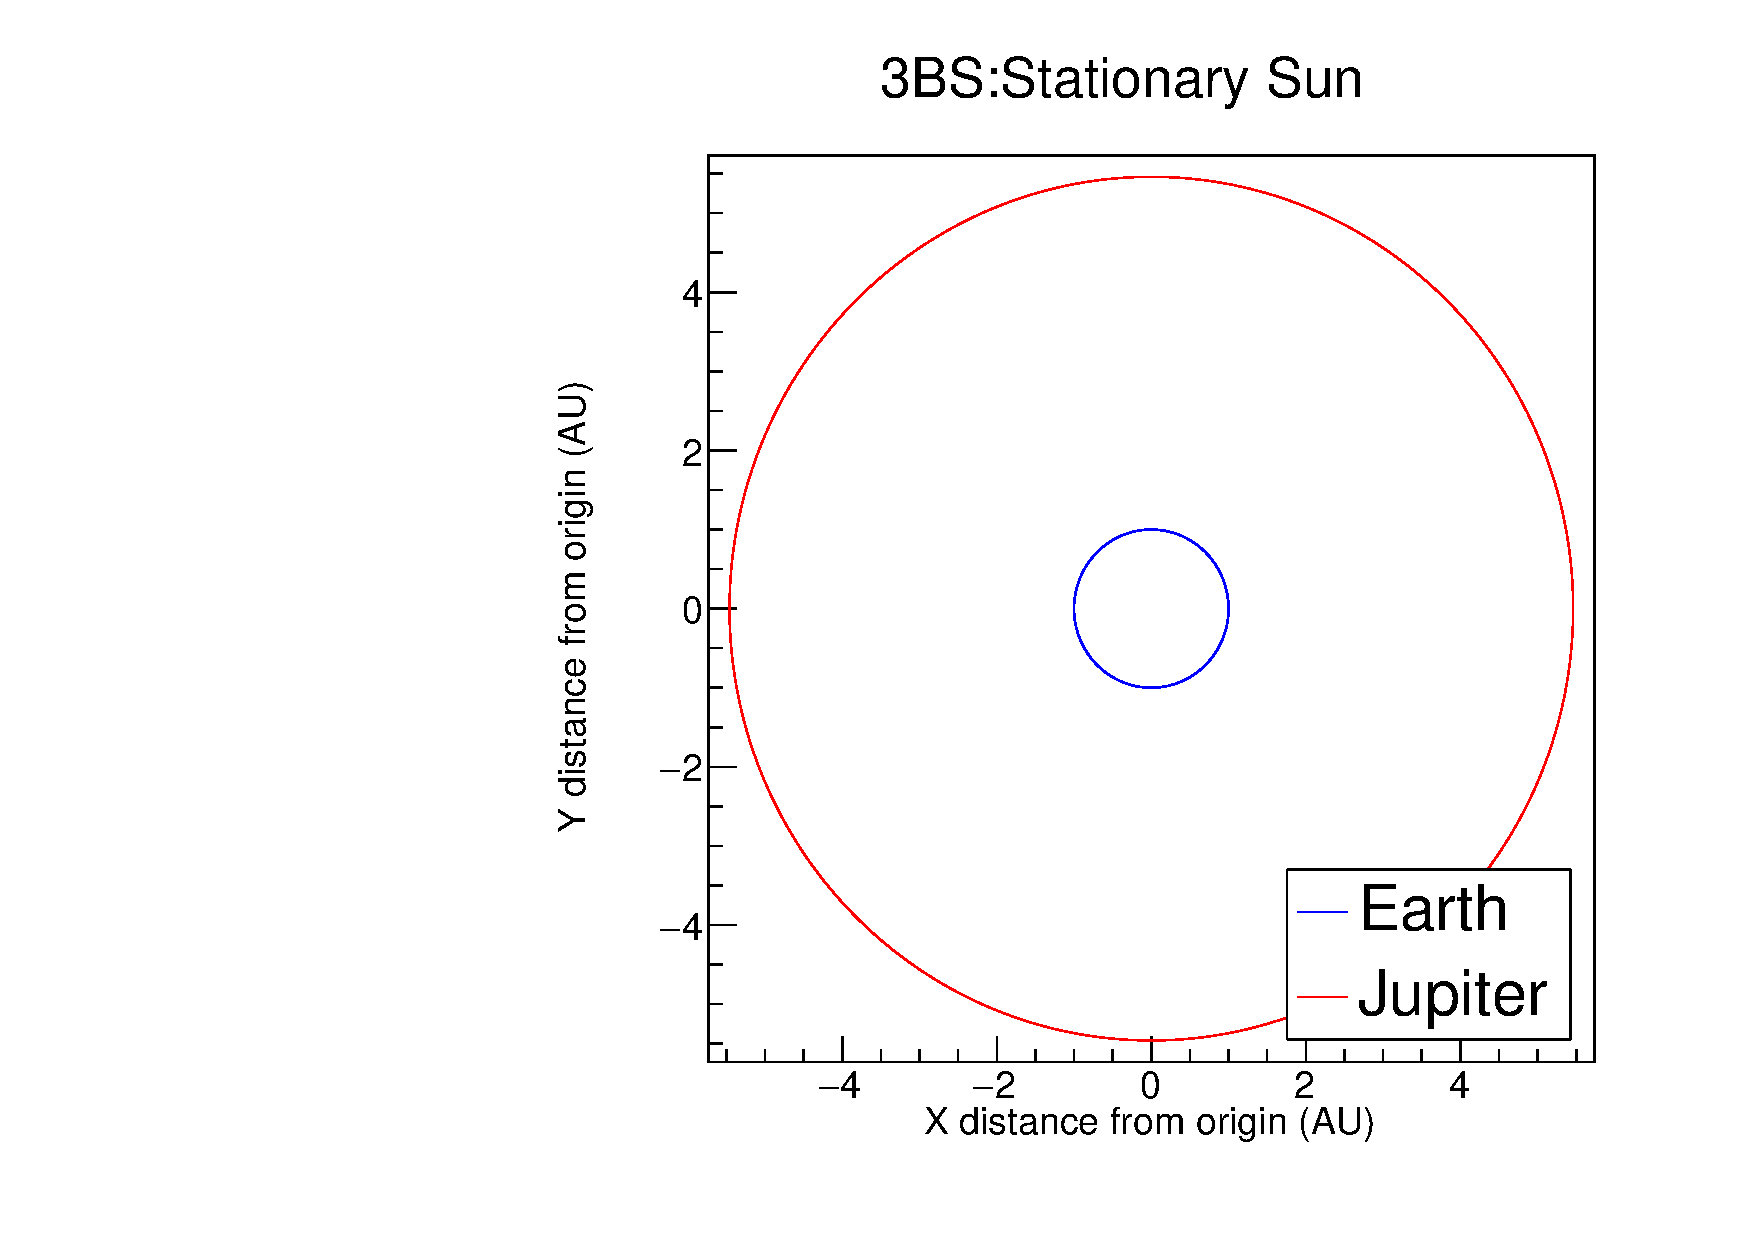
\includegraphics[width=0.5\textwidth]{ESJFVerlet_reg.pdf}
  \caption{Plot of 3 body system with Earth, Jupiter, and a stationary sun using regular Jupiter mass. Time interval: 13 years, Time steps: 13000, Algorithm: Verlet.}
  \label{fig:ESJFVerlet_reg}
 \end{figure}
 
  \begin{figure}[H]
 \centering
   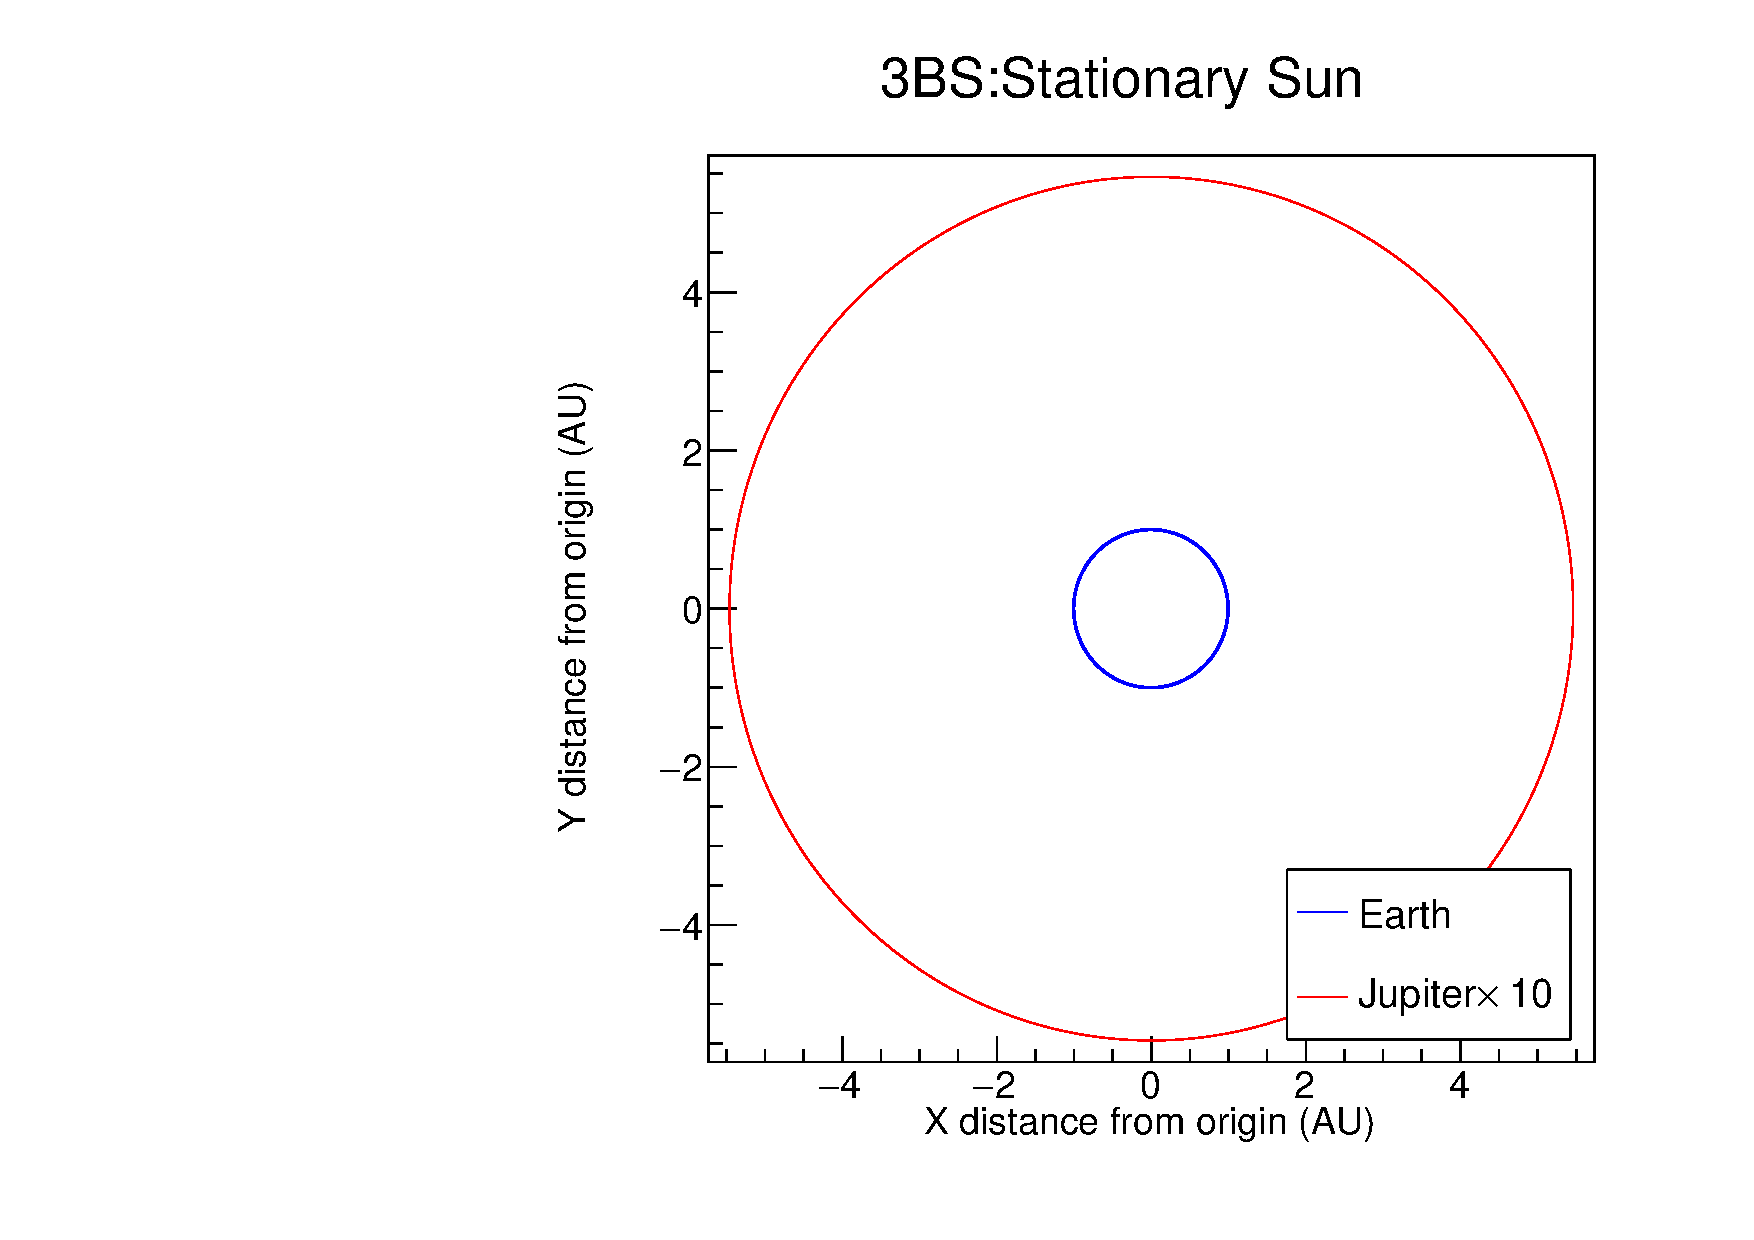
\includegraphics[width=0.5\textwidth]{ESJFVerlet_x10.pdf}
  \caption{Plot of 3 body system with Earth, Jupiter, and a stationary sun using $\times 10$ Jupiter mass. Time interval: 13 years, Time steps: 13000, Algorithm: Verlet.}
  \label{fig:ESJFVerlet_x10}
 \end{figure}
 
  \begin{figure}[H]
 \centering
   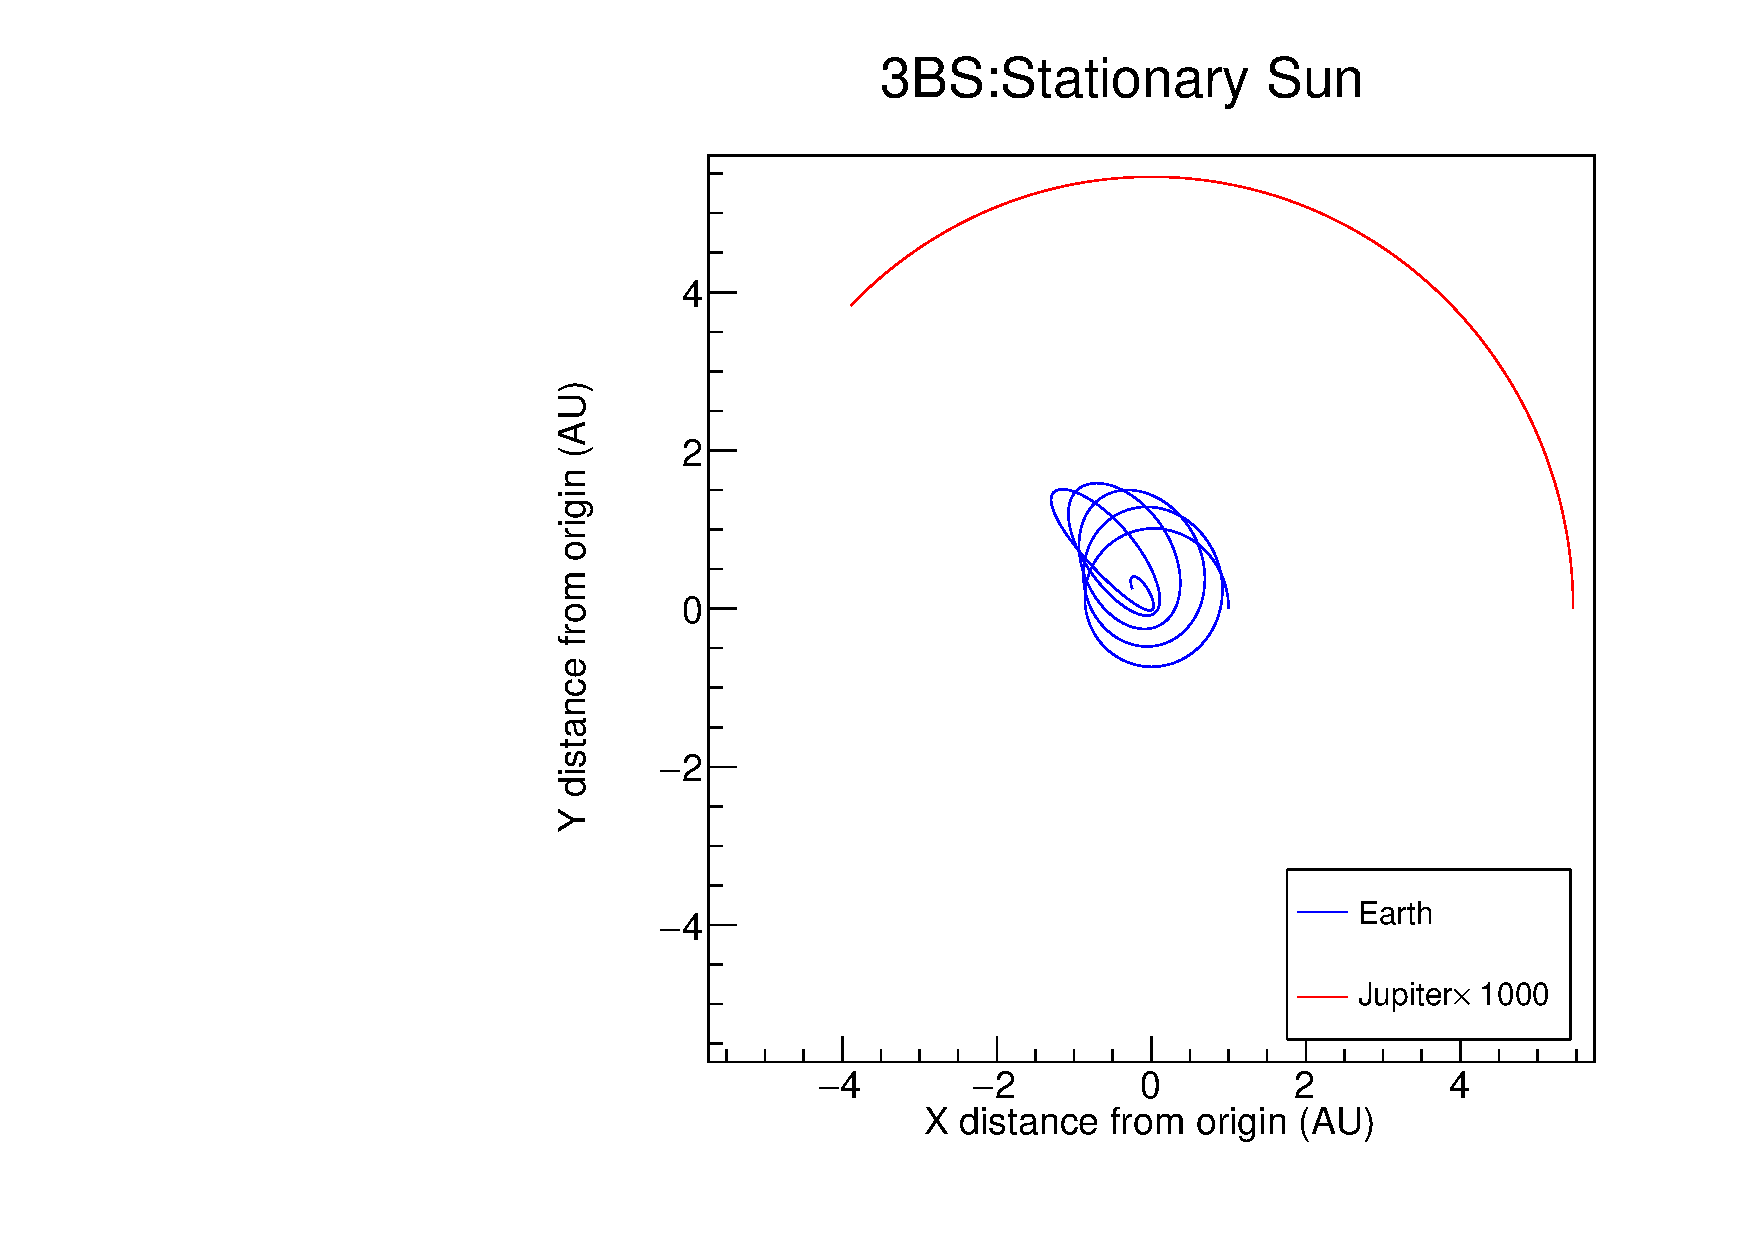
\includegraphics[width=0.5\textwidth]{ESJFVerlet_x1000.pdf}
  \caption{Plot of 3 body system with Earth, Jupiter, and a stationary sun using $\times 1000$ Jupiter mass. Used a shorter timespan because this heavy Jupiter causes Earth to ``hit the sun'', then go barreling out many AU so the orbital structure is no longer visible. Time interval: 4.8 years, Time steps: 13000, Algorithm: Verlet.}
  \label{fig:ESJFVerlet_x1000}
 \end{figure}
 
 \chapter{All RK4 Code}\label{app:rk4}
 \singlespacing
 \begin{Verbatim}[fontsize=\small]
void SolarSystem::RK4(){
  _solved = true;
  double Fx,Fy,Fz;

  for( int i = 1; i <= _Ntime; i++ ){
    vector< vector< double > > k1, k2, k3; 
    for( unsigned int iPlanet = 0; iPlanet < GetN(); iPlanet++ ){

      // Keep planet in same position if it is fixed
      if(_vPlanets.at(iPlanet).Fixed()){
	_vPlanets.at(iPlanet).AddCoordinates(i*_step,
					     _vPlanets.at(iPlanet).X(i-1),
					     _vPlanets.at(iPlanet).Y(i-1),
					     _vPlanets.at(iPlanet).Z(i-1),
					     _vPlanets.at(iPlanet).Vx(i-1),
					     _vPlanets.at(iPlanet).Vy(i-1),
					     _vPlanets.at(iPlanet).Vz(i-1));				    
	vector<double> placeholder;
	k1.push_back(placeholder);
      }
      else{

	// calculate k1
	vector<double> k1i;
	k1i.push_back( _step*_vPlanets.at(iPlanet).Vx(i-1) );
	k1i.push_back( _step*_vPlanets.at(iPlanet).Vy(i-1) );
	k1i.push_back( _step*_vPlanets.at(iPlanet).Vz(i-1) );

	TotalForce(iPlanet,i-1,Fx,Fy,Fz);
	k1i.push_back( _step*Fx/_vPlanets.at(iPlanet).M() );
	k1i.push_back( _step*Fy/_vPlanets.at(iPlanet).M() );
	k1i.push_back( _step*Fz/_vPlanets.at(iPlanet).M() );

	// Advance f(t_i,y_i)->f(t_i+h/2,y_i+k1/2)
	_vPlanets.at(iPlanet).AddCoordinates(i*_step,
					     _vPlanets.at(iPlanet).X(i-1)+k1i.at(0)/2.,
					     _vPlanets.at(iPlanet).Y(i-1)+k1i.at(1)/2.,
					     _vPlanets.at(iPlanet).Z(i-1)+k1i.at(2)/2.,
					     _vPlanets.at(iPlanet).Vx(i-1)+k1i.at(3)/2.,
					     _vPlanets.at(iPlanet).Vy(i-1)+k1i.at(4)/2.,
					     _vPlanets.at(iPlanet).Vz(i-1)+k1i.at(5)/2.);
	k1.push_back(k1i);
      }
    }
    
    for( unsigned int iPlanet = 0; iPlanet < GetN(); iPlanet++ ){
      if(_vPlanets.at(iPlanet).Fixed()){
	vector<double> placeholder;
	k2.push_back(placeholder);
      }
      else{
	// calculate k2
	vector<double> k2i;
	k2i.push_back( _step*_vPlanets.at(iPlanet).Vx(i));
	k2i.push_back( _step*_vPlanets.at(iPlanet).Vy(i));
	k2i.push_back( _step*_vPlanets.at(iPlanet).Vz(i));

	TotalForce(iPlanet,i,Fx,Fy,Fz);
	k2i.push_back( _step*Fx/_vPlanets.at(iPlanet).M() );
	k2i.push_back( _step*Fy/_vPlanets.at(iPlanet).M() );
	k2i.push_back( _step*Fz/_vPlanets.at(iPlanet).M() );

	// Advance f(t_i+h/2,y_i+k1/2)->f(t_i+h/2,y_i+k2/2)
	_vPlanets.at(iPlanet).SetX(_vPlanets.at(iPlanet).X(i-1)+k2i.at(0)/2.,i);
	_vPlanets.at(iPlanet).SetY(_vPlanets.at(iPlanet).Y(i-1)+k2i.at(1)/2.,i);
	_vPlanets.at(iPlanet).SetZ(_vPlanets.at(iPlanet).Z(i-1)+k2i.at(2)/2.,i);
	_vPlanets.at(iPlanet).SetVx(_vPlanets.at(iPlanet).Vx(i-1)+k2i.at(3)/2.,i);
	_vPlanets.at(iPlanet).SetVy(_vPlanets.at(iPlanet).Vy(i-1)+k2i.at(4)/2.,i);
	_vPlanets.at(iPlanet).SetVz(_vPlanets.at(iPlanet).Vz(i-1)+k2i.at(5)/2.,i);
	k2.push_back(k2i);
      }
    }
  
    for( unsigned int iPlanet = 0; iPlanet < GetN(); iPlanet++ ){
      if(_vPlanets.at(iPlanet).Fixed()){
	vector<double> placeholder;
	k3.push_back(placeholder);
      }
      else{
	// calculate k3
	vector<double> k3i;
	k3i.push_back( _step*_vPlanets.at(iPlanet).Vx(i));
	k3i.push_back( _step*_vPlanets.at(iPlanet).Vy(i));
	k3i.push_back( _step*_vPlanets.at(iPlanet).Vz(i));

	TotalForce(iPlanet,i,Fx,Fy,Fz);
	k3i.push_back( _step*Fx/_vPlanets.at(iPlanet).M() );
	k3i.push_back( _step*Fy/_vPlanets.at(iPlanet).M() );
	k3i.push_back( _step*Fz/_vPlanets.at(iPlanet).M() );

	// Advance f(t_i+h/2,y_i+k2/2)->f(t_i+h,y_i+k3)
	_vPlanets.at(iPlanet).SetX(_vPlanets.at(iPlanet).X(i-1)+k3i.at(0),i);
	_vPlanets.at(iPlanet).SetY(_vPlanets.at(iPlanet).Y(i-1)+k3i.at(1),i);
	_vPlanets.at(iPlanet).SetZ(_vPlanets.at(iPlanet).Z(i-1)+k3i.at(2),i);
	_vPlanets.at(iPlanet).SetVx(_vPlanets.at(iPlanet).Vx(i-1)+k3i.at(3),i);
	_vPlanets.at(iPlanet).SetVy(_vPlanets.at(iPlanet).Vy(i-1)+k3i.at(4),i);
	_vPlanets.at(iPlanet).SetVz(_vPlanets.at(iPlanet).Vz(i-1)+k3i.at(5),i);
	k3.push_back(k3i);
      }
    }

    for( unsigned int iPlanet = 0; iPlanet < GetN(); iPlanet++ ){
      if(!_vPlanets.at(iPlanet).Fixed()){
	// calculate k4
	vector<double> k4i;
	k4i.push_back( _step*_vPlanets.at(iPlanet).Vx(i));
	k4i.push_back( _step*_vPlanets.at(iPlanet).Vy(i));
	k4i.push_back( _step*_vPlanets.at(iPlanet).Vz(i));

	Fx = Fy = Fz = 0.;
	TotalForce(iPlanet,i,Fx,Fy,Fz);
	k4i.push_back( _step*Fx/_vPlanets.at(iPlanet).M() );
	k4i.push_back( _step*Fy/_vPlanets.at(iPlanet).M() );
	k4i.push_back( _step*Fz/_vPlanets.at(iPlanet).M() );

	// Advance y_(i+1) = y_i + (1/6)(k1+2k2+2k3+k4)
	_vPlanets.at(iPlanet).SetX(_vPlanets.at(iPlanet).X(i-1)
				   +(k1.at(iPlanet).at(0)
				   +2.*k2.at(iPlanet).at(0)
				   +2.*k3.at(iPlanet).at(0)
				     +k4i.at(0))/6.,i);
	_vPlanets.at(iPlanet).SetY(_vPlanets.at(iPlanet).Y(i-1)
				   +(k1.at(iPlanet).at(1)
				   +2.*k2.at(iPlanet).at(1)
				   +2.*k3.at(iPlanet).at(1)
				     +k4i.at(1))/6.,i);
	_vPlanets.at(iPlanet).SetZ(_vPlanets.at(iPlanet).Z(i-1)
				   +(k1.at(iPlanet).at(2)
				   +2.*k2.at(iPlanet).at(2)
				   +2.*k3.at(iPlanet).at(2)
				     +k4i.at(2))/6.,i);
	_vPlanets.at(iPlanet).SetVx(_vPlanets.at(iPlanet).Vx(i-1)
				    +(k1.at(iPlanet).at(3)
				    +2.*k2.at(iPlanet).at(3)
				    +2.*k3.at(iPlanet).at(3)
				      +k4i.at(3))/6.,i);
	_vPlanets.at(iPlanet).SetVy(_vPlanets.at(iPlanet).Vy(i-1)
				    +(k1.at(iPlanet).at(4)
				    +2.*k2.at(iPlanet).at(4)
				    +2.*k3.at(iPlanet).at(4)
				      +k4i.at(4))/6.,i);
	_vPlanets.at(iPlanet).SetVz(_vPlanets.at(iPlanet).Vz(i-1)
				    +(k1.at(iPlanet).at(5)
				    +2.*k2.at(iPlanet).at(5)
				    +2.*k3.at(iPlanet).at(5)
				      +k4i.at(5))/6.,i);
      }
    }
  }
}
 \end{Verbatim}
 \doublespacing
 
\nocite{*}
\bibliographystyle{plain}
\bibliography{ReportProject3.bib}
\end{document}          
